%%%%%%%%%%%%%%%%%%%%%%%%%%%%%%%%%%%%%%%%%%%%%%%
%%% Template for lab reports used at STIMA
%%%%%%%%%%%%%%%%%%%%%%%%%%%%%%%%%%%%%%%%%%%%%%%

%%%%%%%%%%%%%%%%%%%%%%%%%%%%%% Sets the document class for the document
% Openany is added to remove the book style of starting every new chapter on an odd page (not needed for reports)
\documentclass[11pt,english, openany]{book}

%%%%%%%%%%%%%%%%%%%%%%%%%%%%%% Loading packages that alter the style
\usepackage[]{graphicx}
\usepackage[]{color}
\usepackage{alltt}
\usepackage{amssymb}
\usepackage[T1]{fontenc}
\usepackage[utf8]{inputenc}
\usepackage{amsmath}
\usepackage{blindtext}
\usepackage{tcolorbox}
\usepackage{graphicx}

\setcounter{secnumdepth}{3}
\setcounter{tocdepth}{3}
\setlength{\parskip}{\smallskipamount}
\setlength{\parindent}{0pt}

% Set page margins
\usepackage[top=100pt,bottom=100pt,left=68pt,right=66pt]{geometry}

% Package used for placeholder text
\usepackage{lipsum}

% Prevents LaTeX from filling out a page to the bottom
\raggedbottom

% Adding both languages
\usepackage[english, italian]{babel}

% All page numbers positioned at the bottom of the page
\usepackage{fancyhdr}
\fancyhf{} % clear all header and footers
\fancyfoot[C]{\thepage}
\renewcommand{\headrulewidth}{0pt} % remove the header rule
\pagestyle{fancy}

% Changes the style of chapter headings
\usepackage{titlesec}
\titleformat{\chapter}
   {\normalfont\LARGE\bfseries}{\thechapter.}{1em}{}
% Change distance between chapter header and text
\titlespacing{\chapter}{0pt}{50pt}{2\baselineskip}

% Adds table captions above the table per default
\usepackage{float}
\floatstyle{plaintop}
\restylefloat{table}

% Adds space between caption and table
\usepackage[tableposition=top]{caption}

% Adds hyperlinks to references and ToC
\usepackage{hyperref}
\hypersetup{hidelinks,linkcolor = black} % Changes the link color to black and hides the hideous red border that usually is created

% If multiple images are to be added, a folder (path) with all the images can be added here 
\graphicspath{ {Figures/} }

% Separates the first part of the report/thesis in Roman numerals
\frontmatter


%%%%%%%%%%%%%%%%%%%%%%%%%%%%%% Starts the document
\begin{document}

%%% Selects the language to be used for the first couple of pages
\selectlanguage{english}

%%%%% Adds the title page
\begin{titlepage}
	\clearpage\thispagestyle{empty}
	\centering
	\vspace{1cm}

	% Titles
	% Information about the University
	{\normalsize Universidade Estadual de Campinas\\
		École Centrale de Nantes\\
		Coursera / Pier.\par}
		\vspace{3cm}
	{\Huge \textbf{Machine Learning}} \\
	%\vspace{1cm}
	%{\large \textbf{xxxxx} \par}
	\vspace{4cm}
	{\normalsize Vinícius Cordeiro Pereira\\ % \\ specifies a new line
	             \par}
	\vspace{5cm}
    
%    \centering \includegraphics[scale=0.4]{logo1.pdf}
    
    \vspace{0.5cm}
		
	% Set the date
	{\today \par}
	
	\pagebreak

\end{titlepage}

% Adds a table of contents
\tableofcontents{}

%%%%%%%%%%%%%%%%%%%%%%%%%%%%%%%%%%%%%%%%%%%%%%%%%%%%%%%%%%%%%%%%%%%%%%%%%%%%%%%%%%%%%%%%%%%%
%%%%%%%%%%%%%%%%%%%%%%%%%%%%%%%%%%%%%%%%%%%%%%%%%%%%%%%%%%%%%%%%%%%%%%%%%%%%%%%%%%%%%%%%%%%%
%%%%% Text body starts here!
\mainmatter

\chapter{Introduction}\label{chapt:sum}

\subsection*{What is Machine Learning?}

Two definitions of Machine Learning are offered. 

\begin{enumerate}
\item Arthur Samuel described it as: "\textbf{the field of study that gives computers the ability to learn without being explicitly programmed.}" This is an older, informal definition.

\item Tom Mitchell provides a more modern definition: "\textbf{A computer program is said to learn from experience E with respect to some class of tasks T and performance measure P, if its performance at tasks in T, as measured by P, improves with experience E.}"
\end{enumerate}

Example: playing checkers.

\begin{itemize}
\item E = the experience of playing many games of checkers
\item T = the task of playing checkers.
\item P = the probability that the program will win the next game.
\end{itemize}

In general, any machine learning problem can be assigned to one of two broad classifications: \textit{Supervised learning and Unsupervised learning}.

\subsubsection*{Supervised Learning}

In supervised learning, we are given a data set and already know what our correct output should look like, having the idea that there is a relationship between the input and the output.\\

Supervised learning problems are categorized into "\textbf{regression}" and "\textbf{classification}" problems. In a regression problem, we are trying to predict results within a continuous output, meaning that we are trying to map input variables to some continuous function. In a classification problem, we are instead trying to predict results in a discrete output. In other words, we are trying to map input variables into discrete categories.\\

\pagebreak

Example :\\

Given data about the size of houses on the real estate market, try to predict their price. Price as a function of size is a continuous output, so this is a regression problem.\\

We could turn this example into a classification problem by instead making our output about whether the house "sells for more or less than the asking price." Here we are classifying the houses based on price into two discrete categories.

\subsubsection*{Unsupervised Learning}

Unsupervised learning allows us to approach problems with little or no idea what our results should look like. We can derive structure from data where we don't necessarily know the effect of the variables.\\

We can derive this structure by clustering the data based on relationships among the variables in the data.\\

With unsupervised learning there is no feedback based on the prediction results.\\

Example:\\

Clustering: Take a collection of 1,000,000 different genes, and find a way to automatically group these genes into groups that are somehow similar or related by different variables, such as lifespan, location, roles, and so on.\\

Non-clustering: The "Cocktail Party Algorithm", allows you to find structure in a chaotic environment. (i.e. identifying individual voices and music from a mesh of sounds at a cocktail party).



\chapter{Linear Regression with One Variable}

To establish notation for future use, we’ll use $x^{(i)}$  to denote the “input” variables (living area in this example), also called input features, and $y^{(i)}$ to denote the “output” or target variable that we are trying to predict (price). A pair ($x^{(i)}$, $y^{(i)}$) is called a training example, and the dataset that we’ll be using to learn-a list of m training examples ($x^{(i)}$, $y^{(i)}$); $i=1,...,m$ - is called a\textbf{ training set}. \\

Note that the superscript \textbf{“(i)”} in the notation is simply an index into the training set, and has nothing to do with exponentiation. We will also use X to denote the space of input values, and Y to denote the space of output values. In this example, X = Y = $\mathbb{R}$.\\

To describe the supervised learning problem slightly more formally, our goal is, given a training set, to learn a function h : X $\rightarrow$ Y so that h(x) is a “good” predictor for the corresponding value of y. For historical reasons, this function h is called a hypothesis. Seen pictorially, the process is therefore like this:

\begin{figure}[h!]
	\centering
	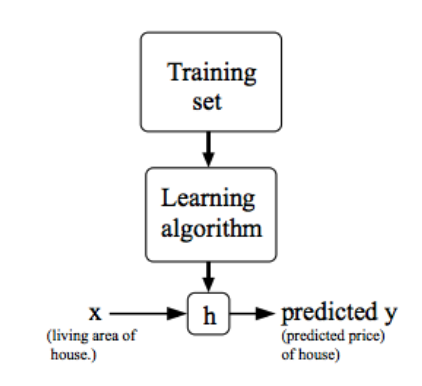
\includegraphics[width=0.5\textwidth]{fig/sl}
	\caption{Supervised learning}
\end{figure}

\section{Cost Function}

We can measure the accuracy of our hypothesis function by using a cost function. This takes an average difference (actually a fancier version of an average) of all the results of the hypothesis with inputs from x's and the actual output y's.

\begin{equation}
J(\theta_0,\theta_1)=\frac{1}{2m}\sum_{i=1}^{m}(\hat{y}_i-y_i)^2 =\frac{1}{2m}\sum_{i=1}^{m}(h_\theta(x_i)-y_i)^2
\end{equation}


Where: 

\begin{center}
$h_\theta(x_i) = \theta_0 + \theta_1\cdot x_i$
\end{center}

This function is otherwise called the "Squared error function", or "Mean squared error". The mean is halved $\left(\frac{1}{2}\right)$  as a convenience for the computation of the gradient descent, as the derivative term of the square function will cancel out the $\frac{1}{2}$ term.\\

\section{Gradient Descent}

So we have our hypothesis function and we have a way of measuring how well it fits into the data. Now we need to estimate the parameters in the hypothesis function. That's where gradient descent comes in.\\

Imagine that we graph our hypothesis function based on its fields $  \theta_0 $ and $ \theta_1 $ (actually we are graphing the cost function as a function of the parameter estimates). We are not graphing x and y itself, but the parameter range of our hypothesis function and the cost resulting from selecting a particular set of parameters.\\

We put $ \theta_0 $ on the x axis and $ \theta_1 $  on the y axis, with the cost function on the vertical z axis. The points on our graph will be the result of the cost function using our hypothesis with those specific theta parameters. The graph below depicts such a setup.\\

\begin{figure}[h!]
	\centering
	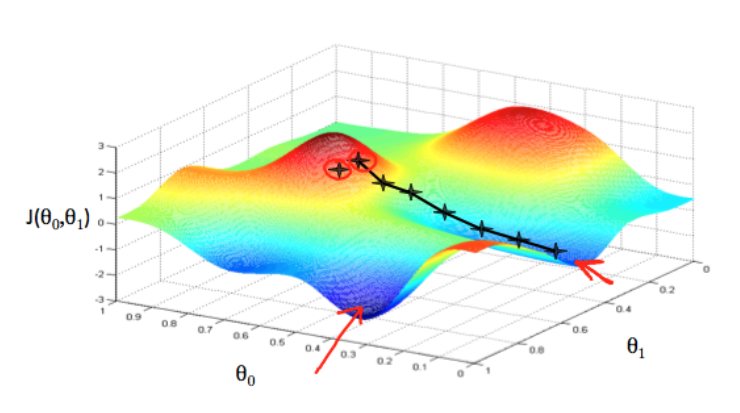
\includegraphics[width=0.8\textwidth]{fig/gradient}
	\caption{Supervised learning}
\end{figure}

\pagebreak

We will know that we have succeeded when our cost function is at the very bottom of the pits in our graph, i.e. when its value is the minimum. The red arrows show the minimum points in the graph.\\

The way we do this is by taking the derivative (the tangential line to a function) of our cost function. The slope of the tangent is the derivative at that point and it will give us a direction to move towards. We make steps down the cost function in the direction with the steepest descent. The size of each step is determined by the parameter $\alpha$, which is called the learning rate.\\

For example, the distance between each 'star' in the graph above represents a step determined by our parameter $\alpha$. A smaller $\alpha$ would result in a smaller step and a larger $\alpha$ results in a larger step. The direction in which the step is taken is determined by the partial derivative of J($ \theta_0 $,$ \theta_1 $). Depending on where one starts on the graph, one could end up at different points. The image above shows us two different starting points that end up in two different places.\\

The gradient descent algorithm is (repeat until convergence):

\begin{equation}
\theta_j := \theta_j - \alpha \frac{\partial}{\partial \theta_j} J(\theta_0, \theta_1) := \theta_j-\alpha \frac{1}{m} \sum_{i=1}^{m}\left(h_\theta(x^{(i)})-y^{(i)}\right)\cdot x^{(i)}_j
\end{equation}

Where, j=0,1 represents the feature index number.\\

\begin{center}
\textbf{Remark :} $\mathbf{ x^{(i)}_0 }$ \textbf{is ALWAYS equal 0.}\\
\end{center}

On a side note, we should adjust our parameter $ \alpha $ to ensure that the gradient descent algorithm converges in a reasonable time. Failure to converge or too much time to obtain the minimum value imply that our step size is wrong.\\

\begin{tcolorbox}[width=\textwidth,colback={lightgray},title={Correct: Simultaneous update},colbacktitle=lightgray,coltitle=blue]    
	$ temp0$ := $ \theta_0 $ - $\alpha \frac{\partial}{\partial \theta_0} J(\theta_0, \theta_1) $ \\
	$ temp1$ := $ \theta_1 $ - $\alpha \frac{\partial}{\partial \theta_1} J(\theta_0, \theta_1) $\\
	$ \theta_0 $ := $ temp0$\\
	$ \theta_1 $ := $ temp1$
\end{tcolorbox} 




\chapter{Linear Regression with Multiple Variables}

Linear regression with multiple variables is also known as "multivariate linear regression".\\

We now introduce notation for equations where we can have any number of input variables.

\begin{itemize}
\item $ x^{(i)}_j $ = value of feature j in the $ i^{th} $ training example
\item $ x^{(i)} $ = the input (features) of the ith training example
\item $ m $ = the number of training examples
\item $ n $ = the number of features
\end{itemize}

The multivariable form of the hypothesis function accommodating these multiple features is as follows:\\

\begin{center}
$h_\theta(x) = \theta_0+\theta_1x_1+\theta_2x_2+\theta_3x_3+ \dots +\theta_nx_n$
\end{center}

In order to develop intuition about this function, we can think about $ \theta_0 $ as the basic price of a house, $ \theta_1 $ as the price per square meter, $ \theta_2 $ as the price per floor, etc. $ x_1 $ will be the number of square meters in the house, $ x_2 $ the number of floors, etc.

Using the definition of matrix multiplication, our multivariable hypothesis function can be concisely represented as:

\begin{align}
h_\theta(x) = \begin{bmatrix}
\theta_{1} \hspace{0.1cm}
\theta_{2} \hspace{0.1cm}
\cdots \hspace{0.1cm}
\theta_{n}
\end{bmatrix}
\begin{bmatrix}
x_{1} \\
x_{2} \\
\vdots \\
x_{n}
\end{bmatrix} = \theta^Tx
\end{align}

\section{Gradient Descent for Multiple Variables}

The gradient descent equation itself is generally the same form; we just have to repeat it for our 'n' features:

\begin{equation}
\theta_j := \theta_j-\alpha \frac{1}{m} \sum_{i=1}^{m}\left(h_\theta(x^{(i)})-y^{(i)}\right)\cdot x^{(i)}_j \hspace{0.7cm} for \hspace{0.1cm} j := 0 \dots n
\end{equation}

\section{Gradient Descent in Practice - Feature Scaling}

We can speed up gradient descent by having each of our input values in roughly the same range. This is because $\theta$ will descend quickly on small ranges and slowly on large ranges, and so will oscillate inefficiently down to the optimum when the variables are very uneven.\\

The way to prevent this is to modify the ranges of our input variables so that they are all roughly the same. Ideally:\\

\begin{center}
-1 $\leq  x_{(i)} \leq $ 1 or -0.5 $ \leq  x_{(i)} \leq $ 0.5
\end{center}

These aren't exact requirements; we are only trying to speed things up. The goal is to get all input variables into roughly one of these ranges, give or take a few.\\

Two techniques to help with this are feature scaling and mean normalization. Feature scaling involves dividing the input values by the range (i.e. the maximum value minus the minimum value) of the input variable, resulting in a new range of just 1. Mean normalization involves subtracting the average value for an input variable from the values for that input variable resulting in a new average value for the input variable of just zero. To implement both of these techniques, adjust your input values as shown in this formula:

\begin{center}
$x_i := \dfrac{x_i - \mu_i}{\sigma_i}$ 
\end{center}

Where $ \mu_i $ is the average of all the values for feature (i) and $ \sigma_i $ is the standard deviation.

\section{Features and Polynomial Regression}

We can improve our features and the form of our hypothesis function in a couple different ways.\\

We can combine multiple features into one. For example, we can combine $ x_1 $ and $ x_2  $ into a new feature $ x_3 $ by taking $ x_1 \cdot  x_2 $.\\

\subsection{Polynomial Regression}

Our hypothesis function need not be linear (a straight line) if that does not fit the data well.\\

We can change the behavior or curve of our hypothesis function by making it a quadratic, cubic or square root function (or any other form).\\

For example, if our hypothesis function is $ h_\theta(x) = \theta_0 + \theta_1 x_1 $ then we can create additional features based on $ x_1 $ to get the quadratic function $ h_\theta(x) = \theta_0 + \theta_1 x_1 + \theta_2 x_1^2 $ or the cubic function $ h_\theta(x) = \theta_0 + \theta_1 x_1 + \theta_2 x_1^2 + \theta_3 x_1^3 $.\\

One important thing to keep in mind is, if you choose your features this way then feature scaling becomes very important.

\section{Normal Equation}

Gradient descent gives one way of minimizing \textbf{J}. Let’s discuss a second way of doing so, this time performing the minimization explicitly and without resorting to an iterative algorithm. In the "\textit{Normal Equation}" method, we will minimize J by explicitly taking its derivatives with respect to the $ \theta_j ’s $, and setting them to zero. This allows us to find the optimum theta without iteration. The normal equation formula is given below:

\begin{equation}
\theta = \left( X^TX\right)^{ -1} X^T y
\end{equation}

There is no need to do feature scaling with the normal equation.\\

\begin{table}[h!]
	\centering
	
	\begin{tabular}{|l|l|}
		\hline
		\textbf{Gradient Descent}  & \textbf{Normal Equation}                      \\ \hline
		Need to choose alpha       & No need to choose alpha                       \\
		Needs many iterations      & No need to iterate                            \\
		$\mathcal{O}$ ($kn^2$)                 & $\mathcal{O}$ ($n^3$), need to calculate inverse of $X^T$ \\
		Works well when n is large & Slow if n is very large                       \\ \hline
	\end{tabular}
\end{table}

With the normal equation, computing the inversion has complexity $\mathcal{O}$($ nˆ3 $). So if we have a very large number of features, the normal equation will be slow. In practice, when n exceeds 10,000 it might be a good time to go from a normal solution to an iterative process.\\

\subsection{Normal Equation Noninvertibility}

When implementing the normal equation in octave we want to use the \textbf{'pinv'} function rather than \textbf{'inv.'} The \textbf{'pinv' }function will give you a value of $ \theta $ even if  $ X^TX $ is not invertible.

If $ X^TX $ is noninvertible, the common causes might be having :

\begin{itemize}
\item Redundant features, where two features are very closely related (i.e. they are linearly dependent)
\item Too many features (e.g. m $ \leq $ n). In this case, delete some features or use "regularization" (to be explained in a later lesson).
\end{itemize}

Solutions to the above problems include deleting a feature that is linearly dependent with another or deleting one or more features when there are too many features.


\chapter{Logistic Regression}

\section{Classification}

The classification problem is just like the regression problem, except that the values we now want to predict take on only a small number of discrete values. For now, we will focus on the binary classification problem in which \textbf{y} can take on only two values, 0 and 1. (Most of what we say here will also generalize to the multiple-class case.) For instance, if we are trying to build a spam classifier for email, then $ x^{(i)} $ may be some features of a piece of email, and y may be 1 if it is a piece of spam mail, and 0 otherwise. Hence, y $\in$ {0,1}. 0 is also called the negative class, and 1 the positive class, and they are sometimes also denoted by the symbols “-” and “+.” Given $ x^{(i)} $, the corresponding $ y^{(i)} $ is also called the label for the training example.

\subsection{Hypothesis Representation}

We could approach the classification problem ignoring the fact that y is discrete-valued, and use our old linear regression algorithm to try to predict y given x. However, it is easy to construct examples where this method performs very poorly. Intuitively, it also doesn’t make sense for $ h_\theta (x) $ to take values larger than 1 or smaller than 0 when we know that y $\in$ {0, 1}. To fix this, let’s change the form for our hypotheses $ h_\theta (x) $ to satisfy $ 0 \leq h_\theta (x) \leq 1 $. This is accomplished by plugging $ \theta^Tx $ into the Logistic Function (also called Sigmoid Function).\\


\begin{tcolorbox}[width=\textwidth,colback={white},colbacktitle=white]
\begin{align*}
h_\theta(x) &=g(\theta^Tx)\\
z &=\theta^Tx\\
g(z) &=\frac{1}{1+e^{-z}}
\end{align*}
\end{tcolorbox} 

\pagebreak

The following image shows us what the sigmoid function looks like:

\begin{figure}[h!]
	\centering
	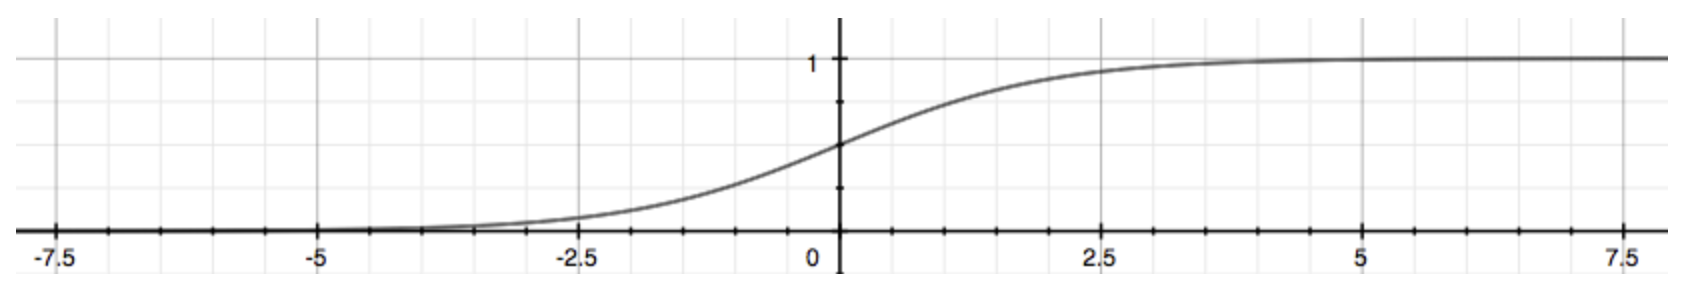
\includegraphics[width=1\textwidth]{fig/sigmoide}
	\caption{Sigmoid function}
\end{figure}

The function $ g(z) $, shown here, maps any real number to the (0, 1) interval, making it useful for transforming an arbitrary-valued function into a function better suited for classification.\\

$\mathbf{ h_\theta(x)  }$ \textbf{will give us the probability that our output is 1.} For example, $ h_\theta(x)=0.7 $ gives us a probability of 70\% that our output is 1. Our probability that our prediction is 0 is just the complement of our probability that it is 1 (e.g. if probability that it is 1 is 70\%, then the probability that it is 0 is 30\%).

\subsection{Decision Boundary}

In order to get our discrete 0 or 1 classification, we can translate the output of the hypothesis function as follows:

\begin{tcolorbox}[width=\textwidth,colback={white},colbacktitle=white]
	\begin{align*}
	When \hspace{0.2cm} z \geq 0  \hspace{0.2cm} \Rightarrow \hspace{0.2cm} h_\theta(x) & \geq 0.5 \rightarrow y=1\\
	When \hspace{0.2cm} z \leq 0  \hspace{0.2cm} \Rightarrow \hspace{0.2cm} h_\theta(x) & \leq 0.5 \rightarrow y=0
	\end{align*}
\end{tcolorbox} 

So if our input to g is $ \theta^T X $, then that means:

\begin{align*}
&h_\theta(x)=g(\theta^Tx) \geq 0.5 \\
&When \hspace{0.2cm} \theta^Tx \geq 0
\end{align*}

From these statements we can now say:

\begin{align*}
\theta^Tx \geq 0 &\Rightarrow y=1\\
\theta^Tx < 0 &\Rightarrow y=0
\end{align*}

The decision boundary is the line that separates the area where \textbf{y = 0 }and where \textbf{y = 1}. It is created by our hypothesis function.

\subsection{Cost Function}

We cannot use the same cost function that we use for linear regression because the Logistic Function will cause the output to be \textbf{wavy}, causing many local optima. In other words, \textit{it will not be a convex function}.

Instead, our cost function for logistic regression looks like:

\begin{equation}
J(\theta)=\frac{1}{m}\sum_{i=1}^{m}Cost\left(h_\theta(x^{(i)}),  y^{(i)}\right)
\end{equation}

Where:

\begin{align}
Cost\left(h_\theta(x^{(i)}),  y^{(i)}\right) &= -log(h_\theta(x)) &if \hspace{0.35cm} y = 1\\
Cost\left(h_\theta(x^{(i)}),  y^{(i)}\right)& = -log(1-h_\theta(x)) & if \hspace{0.35cm} y = 0
\end{align}

\begin{figure}[h!]
	\centering
	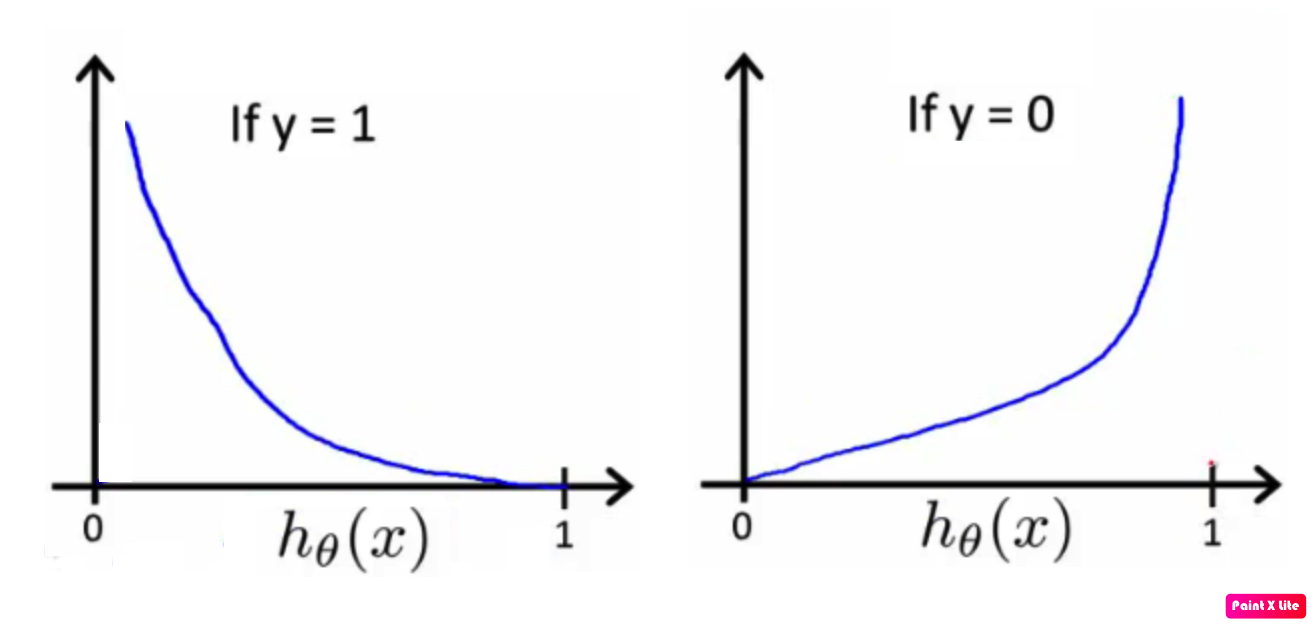
\includegraphics[width=1\textwidth]{fig/cost_logistic}
	\caption{When \textbf{y = 1 (left)}, \textbf{y = 0 (right)} we get the following plot for J($ \theta $) vs $ h_\theta (x) $}
	\label{fig:logistic}
\end{figure}

If our correct answer 'y' is 0, then the cost function will be 0 if our hypothesis function also outputs 0. If our hypothesis approaches 1, then the cost function will approach infinity.\\

If our correct answer 'y' is 1, then the cost function will be 0 if our hypothesis function outputs 1. If our hypothesis approaches 0, then the cost function will approach infinity.\\

We can compress our cost function's two conditional cases into one case:

\begin{equation}
Cost(h_\theta(x^{(i)}),  y^{(i)}) = -y\cdot log(h_\theta(x)) -(1-y)\cdot log(1-h_\theta(x)) 
\end{equation}

We can fully write out our entire cost function as follows:

\begin{center}
$$J(\theta) = -\frac{1}{m}\sum_{i=1}^{m}\left[y^{(i)}\cdot log(h_\theta(x^{(i)})) +(1-y^{(i)})\cdot log(1-h_\theta(x^{(i)}))\right] $$
\end{center}

A vectorized implementation is:

\begin{align*}
h&=g(X\theta) \\
J(\theta)&=\frac{1}{m}\cdot(-y^T\cdot log(h)-(1-y)^T\cdot log(1-h))
\end{align*}

\subsection{Gradient Descent}

The general form of gradient descent is:

\begin{align*}
Repeat &: \{\\
\theta_j &:= \theta_j - \alpha \frac{\partial}{\partial \theta_j} J(\theta_0, \theta_1) \\
 &   \}
\end{align*}

We can work out the derivative part using calculus to get:


\begin{align*}
Repeat &: \{\\
\theta_j &:= \theta_j-\alpha \frac{1}{m} \sum_{i=1}^{m}\left(h_\theta(x^{(i)})-y^{(i)}\right)\cdot x^{(i)}_j \\
&   \}
\end{align*}

\textbf{Notice that this algorithm is identical to the one we used in linear regression. We still have to simultaneously update all values in theta.}\\

A vectorized implementation is:\\

\begin{center}
$\theta:=\theta- \frac{\alpha}{m} X^T \left(g(X\theta)- \overrightarrow{y}\right)$
\end{center}

\section{Multiclass Classification: One-vs-all}

Now we will approach the classification of data when we have more than two categories. Instead of y = {0,1} we will expand our definition so that y = {0,1...n}.\\

Since y = {0,1...n}, we divide our problem into n+1 (+1 because the index starts at 0) binary classification problems; in each one, we predict the probability that 'y' is a member of one of our classes.\\

\begin{tcolorbox}[width=\textwidth,colback={white},colbacktitle=white]
	\begin{align*}
	&y \in \{0,1 \dots n\}\\
	&h^{(0)}_\theta(x)=P(y=0|x;\theta)\\
	&h^{(1)}_\theta(x)=P(y=1|x;\theta)\\
	&\dots\\
	&h^{(n)}_\theta(x)=P(y=n|x;\theta)\\
	&prediction = \underset{i}max(h^{(i)}_\theta(x))
	\end{align*}
\end{tcolorbox} 

We are basically choosing one class and then lumping all the others into a single second class. We do this repeatedly, applying binary logistic regression to each case, and then use the hypothesis that returned the highest value as our prediction.\\

The following image shows how one could classify 3 classes:\\

\begin{figure}[h!]
	\centering
	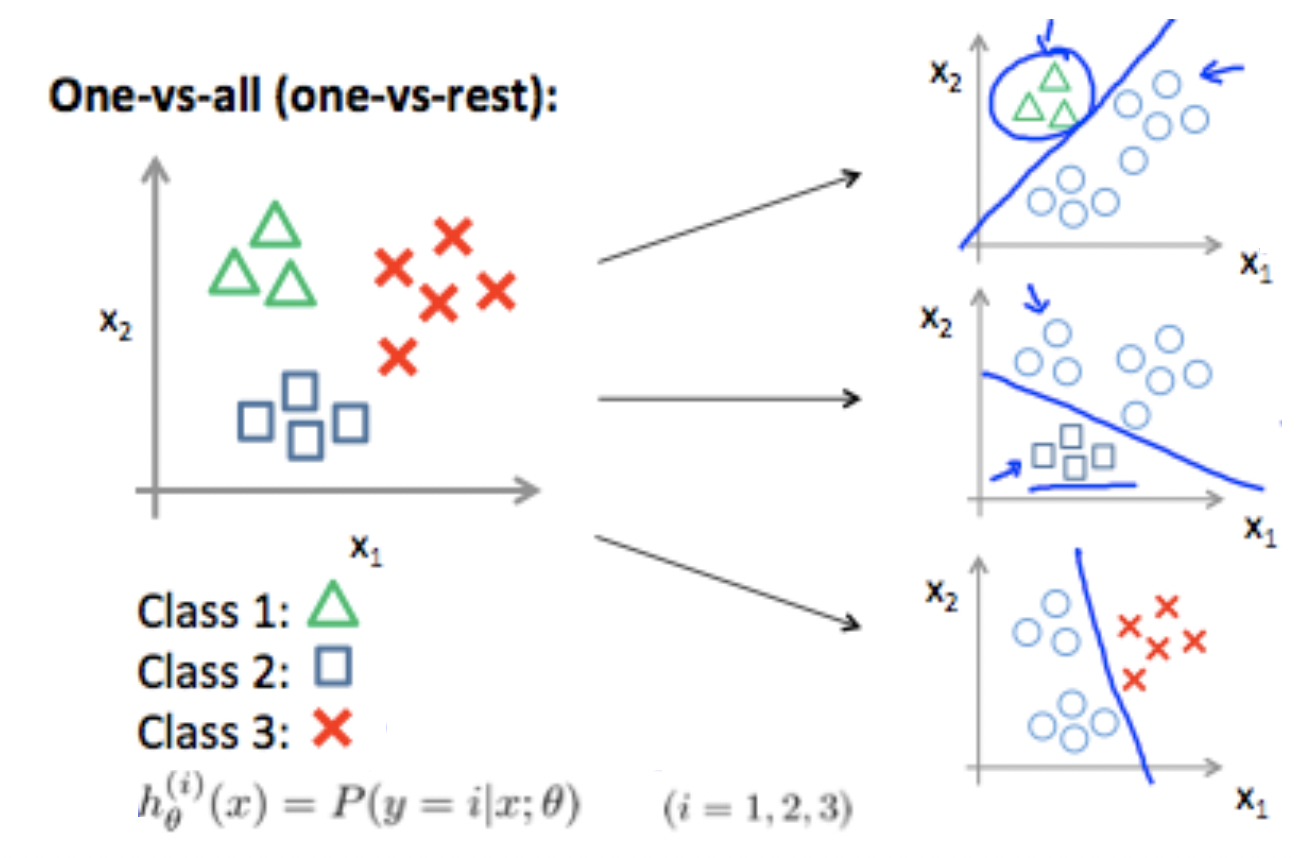
\includegraphics[width=0.65\textwidth]{fig/onvsall}
	\caption{One-vs-all or One-vs-Rest}
\end{figure}

\chapter{Regularization}

\section{The Problem of Overfitting}

Consider the problem of predicting y from x $\in$ $ \mathbb{R} $. The leftmost figure below shows the result of fitting a $ y = \theta_0+\theta_1x $ to a dataset. We see that the data doesn’t really lie on straight line, and so the fit is not very good.\\

Instead, if we had added an extra feature $ x^2 $, and fit $ y = \theta_0 + \theta_1x + \theta_2x^2 $, then we obtain a slightly better fit to the data (See middle figure). Naively, it might seem that the more features we add, the better. However, there is also a danger in adding too many features: The rightmost figure is the result of fitting a $ 5^{th} $order polynomial $$ y = \sum_{j=0} ^5 \theta_j x^j .$$ We see that even though the fitted curve passes through the data perfectly, we would not expect this to be a very good predictor of, say, housing prices (y) for different living areas (x). Without formally defining what these terms mean, we’ll say the \textit{figure on the left} shows an instance of \textbf{underfitting}—in which the data clearly shows structure not captured by the model—and the \textit{figure on the right} is an example of \textbf{overfitting}.

\begin{figure}[h!]
	\centering
	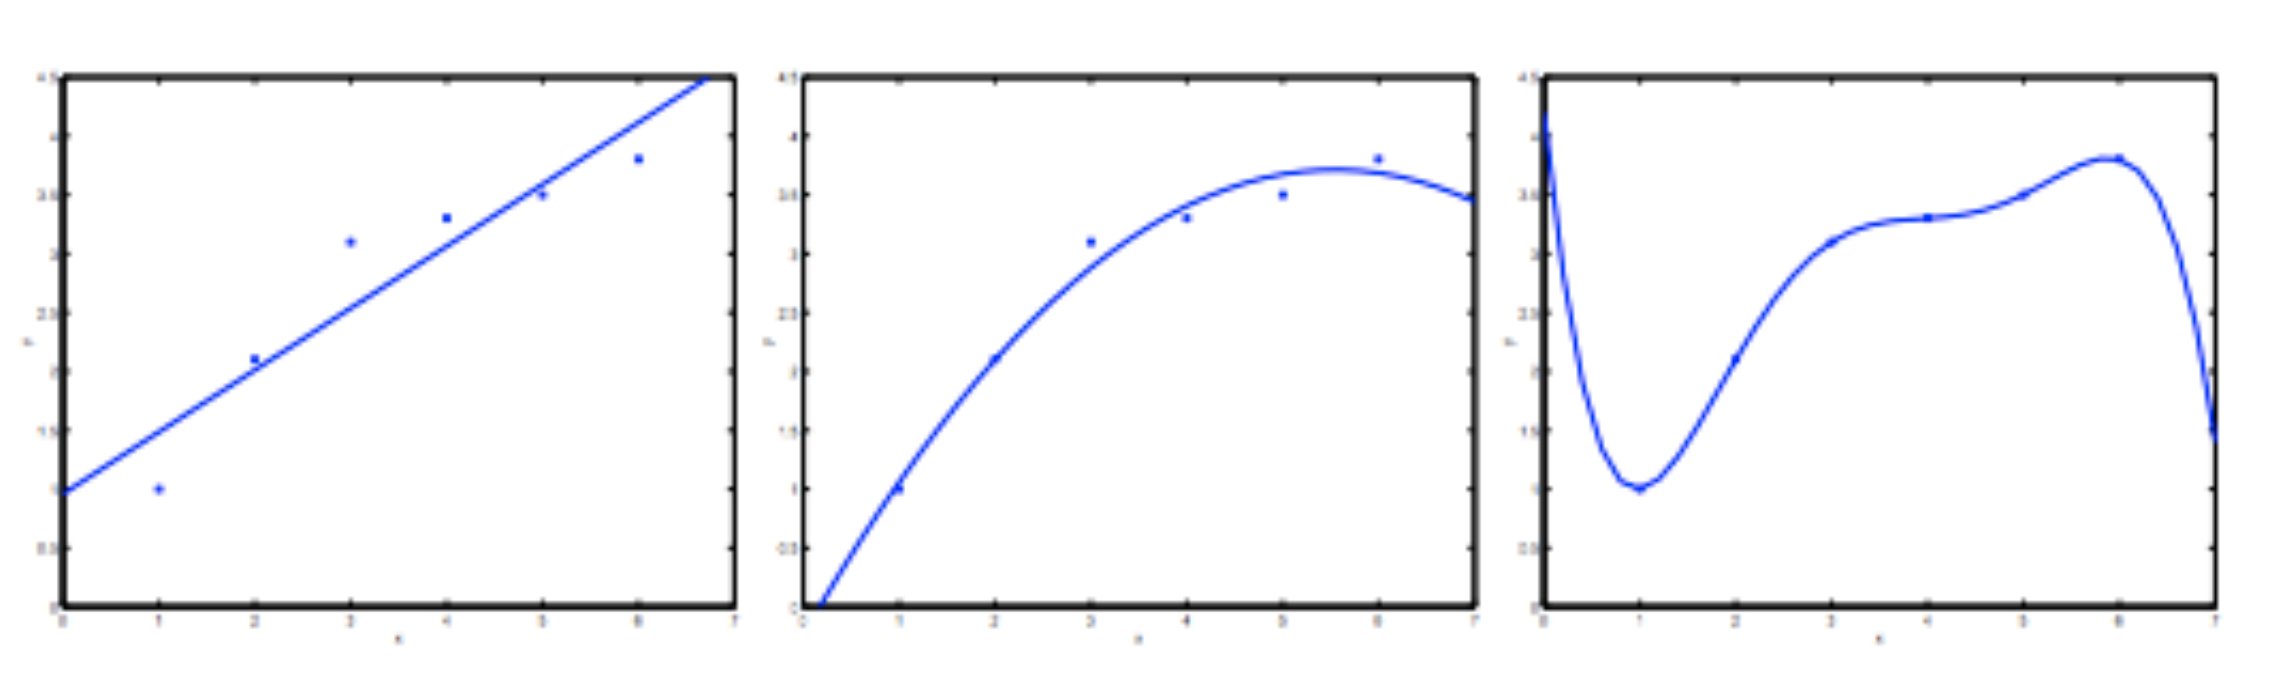
\includegraphics[width=1\textwidth]{fig/regula}
	\caption{One-vs-all or One-vs-Rest}
\end{figure}

\textbf{Underfitting, or high bias}, is when the form of our hypothesis function h maps poorly to the trend of the data.\\

\textbf{Overfitting, or high variance}, is caused by a hypothesis function that fits the available data but does not generalize well to predict new data.\\

This terminology is applied to both linear and logistic regression. There are two main options to address the issue of overfitting:\\

\begin{enumerate}
\item Reduce the number of features: Manually select which features to keep; Use a model selection algorithm.
\item Regularization: Keep all the features, but reduce the magnitude of parameters $ \theta_j $. Regularization works well when we have a lot of slightly useful features.
\end{enumerate}

\section{Cost Function}

Say we wanted to make the following function more quadratic:

\begin{center}
$ y = \theta_0 + \theta_1x + \theta_2x^2 + \theta_3x^3 + \theta_4x^4$
\end{center}

We'll want to eliminate the influence of $ \theta_3x^3 $and $ \theta_4x^4 $ without actually getting rid of these features or changing the form of our hypothesis, we can instead modify our cost function:\\

\begin{center}
$$min_\theta   \frac{1}{2m}\sum_{i=1}^{m}\left(h_\theta(x^{(i)}) - y^{(i)}\right)^2 + 1000\cdot \theta_3x^3 + 1000\cdot \theta_4x^4 $$
\end{center}

We've added two extra terms at the end to inflate the cost of $ \theta_3 $and $ \theta_4 $. Now, in order for the cost function to get close to zero, we will have to reduce the values of $ \theta_3 $and $ \theta_4 $ to near zero. This will in turn greatly reduce the values of $ \theta_3 x^3 $and $ \theta_4x^4 $ in our hypothesis function.\\

\subsection{Linear Regression}

We could also regularize all of our theta parameters in a single summation as:\\

\begin{center}
	$$min_\theta   \frac{1}{2m}\sum_{i=1}^{m}\left(h_\theta(x^{(i)}) - y^{(i)}\right)^2 + \lambda  \sum_{i=1}^{n} \theta_j^2$$
\end{center}

The lambda is the regularization parameter. It determines how much the costs of our theta parameters are inflated.

\subsection{Logistic Regression}

\begin{center}
	$$J(\theta) = -\frac{1}{m}\sum_{i=1}^{m}\left[y^{(i)}\cdot log(h_\theta(x^{(i)})) +(1-y^{(i)})\cdot log(1-h_\theta(x^{(i)}))\right] + \frac{\lambda}{2m}  \sum_{i=1}^{n} \theta_j^2$$
\end{center}

The second sum, $$\sum_{i=1}^{n} \theta_j^2$$ means to explicitly exclude the bias term, $ \theta_0 $. I.e. the $ \theta $ vector is indexed from 0 to n (holding n+1 values, $ \theta_0 $ through $ \theta_n $), and this sum explicitly skips $ \theta_0 $, by running from 1 to n, skipping 0. (\textbf{Identically for linear regression}).

\section{Gradient Descent}

We will modify our gradient descent function to separate out $ \theta_0 $ from the rest of the parameters because we do not want to penalize $ \theta_0 $.

\begin{align*}
Repeat &: \{\\
\theta_0 &:= \theta_0-\alpha \frac{1}{m} \sum_{i=1}^{m}\left(h_\theta(x^{(i)})-y^{(i)}\right)\cdot x^{(i)}_0\\
\theta_j &:= \theta_j-\alpha \left[ \left(\frac{1}{m} \sum_{i=1}^{m}\left(h_\theta(x^{(i)})-y^{(i)}\right)\cdot x^{(i)}_j  \right) +\frac{\lambda}{m}\theta_j\right] \hspace{1cm} j \in \{1,2, \dots, n\}\\
&   \}
\end{align*}

\section{Normal Equation}

Now let's approach regularization using the alternate method of the non-iterative normal equation.\\

To add in regularization, the equation is the same as our original, except that we add another term inside the parentheses:\\

\begin{center}
$\theta = (X^TX+\lambda\cdot L)^{-1} X^Ty$
\end{center}

Where:

\[
L =
\begin{bmatrix}
0 & && &\\
& 1& & &\\
& & 1&&\\
&&&\ddots&\\
&&&&1
\end{bmatrix}
\]

L is a matrix with 0 at the top left and 1's down the diagonal, with 0's everywhere else. It should have dimension (n+1)x(n+1).

\chapter{Neural Networks}

Neural networks are a set of algorithms, modeled loosely after the human brain, that are designed to recognize patterns. They interpret sensory data through a kind of machine perception, labeling or clustering raw input. The patterns they recognize are numerical, contained in vectors, into which all real-world data, be it images, sound, text or time series, must be translated.\\

Neural networks help us cluster and classify. You can think of them as a clustering and classification layer on top of the data you store and manage. They help to group unlabeled data according to similarities among the example inputs, and they classify data when they have a labeled dataset to train on. \\

\section{Model Representation}

Let's examine how we will represent a hypothesis function using neural networks. At a very simple level, neurons are basically computational units that take inputs (dendrites) as electrical inputs (called "spikes") that are channeled to outputs (axons). In our model, our dendrites are like the input features $x_1\dots x_n$, and the output is the result of our hypothesis function. In this model our $ x_0 $ input node is sometimes called the "bias unit." It is always equal to 1. In neural networks, we use the same logistic function as in classification, $ \frac{1}{1 + e^{-\theta^Tx}} $, yet we sometimes call it a sigmoid (logistic) activation function. In this situation, our "theta" parameters are sometimes called "weights".\\

\begin{figure}[h!]
	\centering
	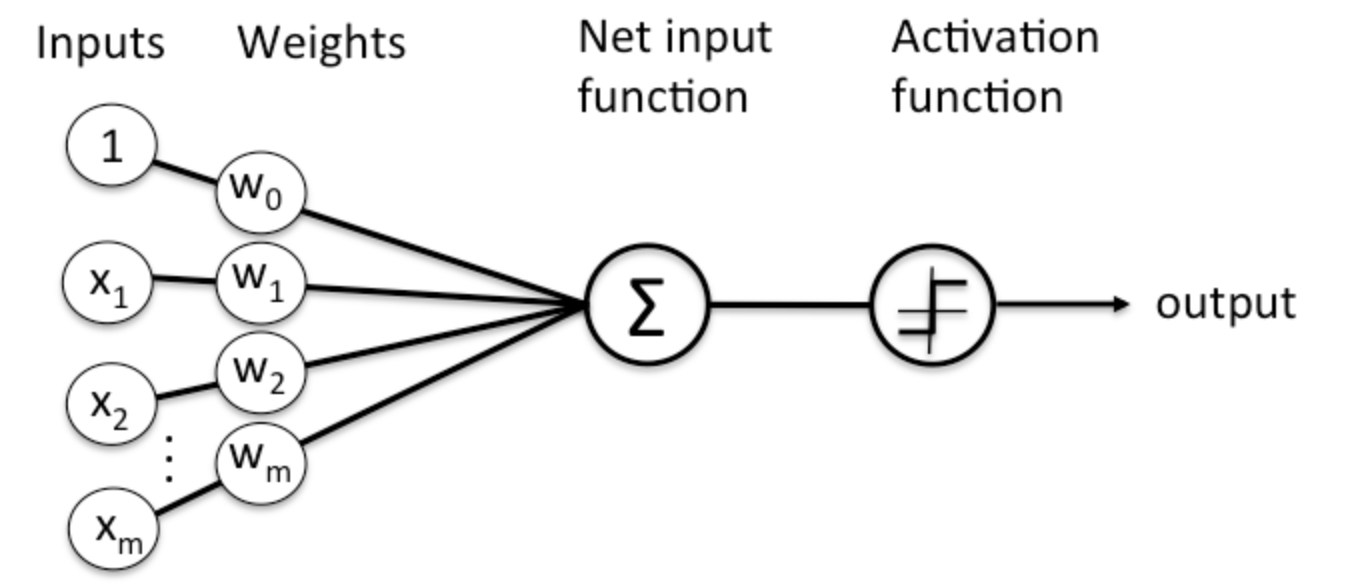
\includegraphics[width=0.7\textwidth]{fig/neural_diag}
	\caption{Neural diagram}
\end{figure}

\pagebreak

Visually, a simplistic representation looks like:\\

\begin{align*}
\begin{bmatrix}
x_{1} \\
x_{2} \\
\vdots \\
x_{n}
\end{bmatrix}
\rightarrow
[ \hspace{0.5cm}]
\rightarrow  h_\theta (x)
\end{align*}

Our input nodes (layer 1), also known as the "input layer", go into another node (layer 2), which finally outputs the hypothesis function, known as the "output layer".We can have intermediate layers of nodes between the input and output layers called the "hidden layers."

\begin{figure}[h!]
	\centering
	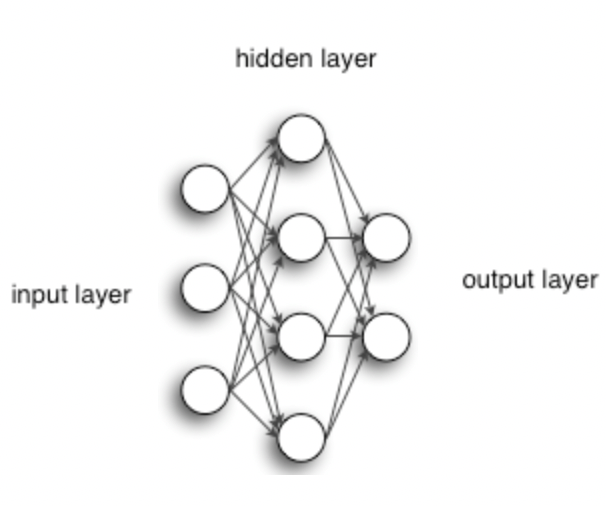
\includegraphics[width=0.5\textwidth]{fig/neural_net}
	\caption{Neural layers}
\end{figure}

Where:

\begin{itemize}
\item $ a^{(j)}_i $ = "\textbf{activation}" of unit \textit{i} in layer \textit{j}\\
\item $\Theta ^{(j)} $=matrix of \textbf{weights} controlling function mapping from layer \textit{j} to layer \textit{j+1}
\end{itemize}

If we had one hidden layer, with \textbf{3} activations,  it would look like:

\begin{align*}
\begin{bmatrix}
x_{0}\\
x_{1} \\
x_{2} \\
x_{3}
\end{bmatrix}
\rightarrow
\begin{bmatrix}
\vspace{0.15cm}a_{1}^{(2)}\\\vspace{0.15cm}
a_{2}^{(2)} \\
a_{3}^{(2)}
\end{bmatrix}
\rightarrow  h_\theta (x)
\end{align*}

The values for each of the "activation" nodes is obtained as follows:

\begin{align*}
a^{(2)}_1&=g\left(\Theta^{(1)}_{10}x_0+\Theta^{(1)}_{11}x_1+\Theta^{(1)}_{12}x_2+\Theta^{(1)}_{13}x_3\right)\\
a^{(2)}_2&=g\left(\Theta^{(1)}_{20}x_0+\Theta^{(1)}_{21}x_1+\Theta^{(1)}_{22}x_2+\Theta^{(1)}_{23}x_3\right)\\
a^{(2)}_3&=g\left(\Theta^{(1)}_{30}x_0+\Theta^{(1)}_{31}x_1+\Theta^{(1)}_{32}x_2+\Theta^{(1)}_{33}x_3\right)\\
h\Theta^(x_)=a^{(3)} _1&=g\left(\Theta^{(2)}_{10}a^{(2)}_0+\Theta^{(2)}_{11}a^{(2)}_1+\Theta^{(2)}_{12}a^{(2)}_2+\Theta^{(2)}_{13}a^{(2)}_3\right)
\end{align*}

This is saying that we compute our activation nodes by using a \textit{3x4} matrix of parameters. We apply each row of the parameters to our inputs to obtain the value for one activation node. Our hypothesis output is the logistic function applied to the sum of the values of our activation nodes, which have been multiplied by yet another parameter matrix $ \Theta ˆ{(2)} $ containing the weights for our second layer of nodes. And each layer gets its own matrix of weights, $ \Theta ^{(j)} $.\\

The dimensions of these matrices of weights is determined as follows:\\

\begin{tcolorbox}[width=\textwidth,colback={white},colbacktitle=white]
If network has $ s_j $ units in layer $ j $ and $ s_{j+1} $  units in layer $ j+1 $, then $ \Theta^{(j)} $ will be of dimension $ s_{j+1} \times (s_j+1) $.
\end{tcolorbox}

\vspace{0.5cm}

The \textbf{+1} comes from the addition in $ \Theta ^{(j)} $ of the "\textbf{bias nodes}", $ x_0 $ and $ \Theta ^{(j)}_0 $. In other words the output nodes will not include the bias nodes while the inputs will.

\subsection{Vectorized implementation}

We're going to define a new variable $ z_k^{(j)} $ that encompasses the parameters inside our \textbf{g} function. In our previous example if we replaced by the variable \textbf{z} for all the parameters we would get:

\begin{align*}
a^{(2)}_1&=g\left(z^{(2)}_1  \right)\\
a^{(2)}_2&=g\left(z^{(2)}_2  \right)\\
a^{(2)}_3&=g\left(z^{(2)}_3  \right)
\end{align*}

In other words, for layer $ j=2 $ and node \textbf{k}, the variable \textbf{z} will be:

\begin{center}
$z^{(2)}_k=g\left(\Theta^{(1)}_{k,0}x_0+\Theta^{(1)}_{k,1}x_1+ \dots +\Theta^{(1)}_{k,n}x_n\right)$
\end{center}

Setting the input $ x = a^{(1)} $, we can rewrite the equation as:

\begin{equation}
z^{(j)} = \Theta^{(j-1)}  a^{(j-1)}  
\end{equation}

Now we can get a vector of our activation nodes for layer j as follows:

\begin{equation}
a^{(j)}  = g(z^{(j)})
\end{equation}

\section{Cost Function}

Let's first define a few variables that we will need to use:

\begin{itemize}
\item $ L $ = total number of layers in the network
\item $ s_l $ = number of units (not counting bias unit) in layer l
\item $ K $ = number of output units/classes
\end{itemize}

Our cost function for neural networks is going to be a generalization of the one we used for logistic regression, but it is going to be slightly more complicated:

\begin{center}
$$J(\theta) = 
-\frac{1}{m}\sum_{i=1}^{m} \sum_{k=1}^{K} 
\left[
y^{(i)}_k\cdot log((h_\theta(x^{(i)}))_k) 
+(1-y^{(i)}_k)\cdot log(1-(h_\theta(x^{(i)}))_k)
\right] 
+ \frac{\lambda}{2m}  
\sum_{l=1}^{L-1}
\sum_{i=1}^{s_j}
\sum_{j=1}^{s_{j+1}} 
\left(
\Theta_{j,i}^{(l)}
\right)^2
$$
\end{center}

We have added a few nested summations to account for our multiple output nodes. In the first part of the equation, before the square brackets, we have an additional nested summation that loops through the number of output nodes.\\

In the regularization part, after the square brackets, we must account for multiple theta matrices. The number of columns in our current theta matrix is equal to the number of nodes in our current layer (including the bias unit). The number of rows in our current theta matrix is equal to the number of nodes in the next layer (excluding the bias unit). As before with logistic regression, we square every term.\\

Note:

\begin{itemize}
\item the double sum simply adds up the logistic regression costs calculated for each cell in the output layer
\item the triple sum simply adds up the squares of all the individual $ \Theta s $ in the entire network.
\item the i in the triple sum does not refer to training example i
\end{itemize}

\section{Backpropagation Algorithm}

"Backpropagation" is neural-network terminology for \textbf{minimizing our cost function}, just like what we were doing with gradient descent in logistic and linear regression. Our goal is to compute:

\begin{center}
	$ min_\Theta J(\Theta) $
\end{center}

To do so, we use the following algorithm:\\

Given training set $ {(x^{(1)},y^{(1)}) \dots (x^{(m)},y^{(m)})} $\\

Set $ \Delta^{(l)}_{i,j} := 0 $ for all $ (l,i,j) $, (hence you end up having a matrix full of zeros).\\

For training example t =1 to m:\\

\begin{enumerate}
\item Set $ a^{(1)} := x^{(t)} $\\

\item Perform forward propagation to compute $ a^{(l)} $, for l=2,3,…,L\\

\item Using $ y^{(t)} $, compute $ \delta^{(L)} = a^{(L)} - y^{(t)} $\\

Where L is our total number of layers and $ a^{(L)} $ is the vector of outputs of the activation units for the last layer. So our "error values" for the last layer are simply the differences of our actual results in the last layer and the correct outputs in \textbf{y}. To get the delta values of the layers before the last layer, we can use an equation that steps us back from right to left:\\

\item Compute $ \delta^{(L-1)} $, $ \delta^{(L-2)} $,$ \dots $,$ \delta^{(2)} $ using $ \delta^{(l)}=((\Theta^{(l)})^T\delta^{(l+1)}) .* a^{(l)} .* (1-a^{(l)}) $\\

The delta values of layer l are calculated by multiplying the delta values in the next layer with the theta matrix of layer l. We then element-wise multiply that with a function called g', or g-prime, which is the derivative of the activation function g evaluated with the input values given by $ z^{(l)} $\\

The g-prime derivative terms can also be written out as:

\begin{center}
$g'(z ^{(l)})= a ^{(l)}.* (1-a ^{(l)})$
\end{center}

\pagebreak

\item $ \Delta^{(l)}_{i,j} := \Delta^{(l)}_{i,j} + a^{(l)}_j \delta^{(l+1)}$ or with vectorization, $ \Delta^{(l)} := \Delta^{(l)} + \delta^{(l+1)}(a^{(l)})^T $\\

Hence we update our new $ \Delta $ matrix.

\begin{itemize}
\item $D _{i,j}^{(l)} := \frac{1}{m} \left(\Delta^{(l)}_{i,j} + \lambda \Theta ^{(l)}_{i,j}\right), \hspace{0.5cm} if \hspace{0.2cm} j \neq 0.$
\item $D _{i,j}^{(l)} := \frac{1}{m} \Delta^{(l)}_{i,j}, \hspace{2.4cm} if \hspace{0.2cm}j = 0.$
\end{itemize}

The capital-delta matrix D is used as an "accumulator" to add up our values as we go along and eventually compute our partial derivative. Thus we get $\frac{\partial}{\partial \Theta} ^{(l)}_{ij}J(\Theta) =  D_{ij}^{(l)} $
\end{enumerate}



\chapter{Advice for Applying Machine Learning}

\section{Evaluating a Hypothesis}

Once we have done some trouble shooting for errors in our predictions by:
\begin{itemize}
\item Getting more training examples
\item Trying smaller sets of features
\item Trying additional features
\item Trying polynomial features
\item Increasing or decreasing $\lambda$
\end{itemize}

We can move on to evaluate our new hypothesis.\\

A hypothesis may have a low error for the training examples but still be inaccurate (because of overfitting). Thus, to evaluate a hypothesis, given a dataset of training examples, we can split up the data into two sets: a training set and a test set. Typically, the training set consists of 70 \% of your data and the test set is the remaining 30 \%.\\

The new procedure using these two sets is then:\\

\begin{enumerate}
\item Learn $\Theta$ and minimize $J_{train}(\Theta)$ using the training set.
\item Compute the test set error $J_{test}(\Theta)$
\end{enumerate}

\subsection{The test set error}

\begin{enumerate}
\item For linear regression: $$J_{test} (\Theta) =\frac{1}{2m_{test}}\sum_{i=1}^{m_{test}}(h_\Theta(x^{(i)}_{test})-y^{(i)}_{test})^2 $$

\item For classification $\rightarrow$ Misclassification error (aka 0/1 misclassification error):

\begin{center}
$err(h_\Theta(x),y) = \begin{cases} 1, & \mbox{if } h_\Theta(x) \geq 0.5  \mbox{ and } y=0 \mbox{ or } h_\Theta(x) < 0.5 \mbox{ and } y=1 \\ 0, & \mbox{otherwise } \end{cases}$
\end{center}
\end{enumerate}

This gives us a binary 0 or 1 error result based on a misclassification. The average test error for the test set is:

\begin{center}
$$\mbox{Test Error = } \frac{1}{m_{test}}\sum_{i=1}^{m_{test}}err(h_\Theta(x^{(i)}_{test})-y^{(i)}_{test})$$
\end{center}

This gives us the proportion of the test data that was misclassified.


\section{Model Selection and Train/Validation/Test Sets}

Just because a learning algorithm fits a training set well, that does not mean it is a good hypothesis. It could over fit and as a result your predictions on the test set would be poor. The error of your hypothesis as measured on the data set with which you trained the parameters will be lower than the error on any other data set.\\

Given many models with different polynomial degrees, we can use a systematic approach to identify the 'best' function. In order to choose the model of your hypothesis, you can test each degree of polynomial and look at the error result.\\

One way to break down our dataset into the three sets is:

\begin{itemize}
\item Training set: 60\%
\item Cross validation set: 20\%
\item Test set: 20\%
\end{itemize}

We can now calculate three separate error values for the three different sets using the following method:

\begin{enumerate}
\item Optimize the parameters in $\Theta$ using the training set for each polynomial degree.
\item Find the polynomial degree \textit{d} with the least error using the cross validation set.
\item Estimate the generalization error using the test set with $ J_{test}(\Theta^{(d)}) $, (\textit{d }= theta from polynomial with lower error);
\end{enumerate}

This way, the degree of the polynomial \textit{d} has not been trained using the test set.

\section{Diagnosing Bias vs. Variance}

In this section we examine the relationship between the degree of the polynomial \textit{d} and the underfitting or overfitting of our hypothesis.\\

We need to distinguish whether bias or variance is the problem contributing to bad predictions, given that \textbf{high bias is underfitting} and \textbf{high variance is overfitting}. Ideally, we need to find a golden mean between these two.\\

The training error will tend to decrease as we increase the degree \textit{d} of the polynomial. At the same time, the cross validation error will tend to decrease as we increase \textit{d} up to a point, and then it will increase as \textit{d} is increased, forming a convex curve.\\

\begin{tcolorbox}[width=\textwidth,colback={white},colbacktitle=white]
\textbf{High bias (underfitting)}: both $ J_{train}(\Theta) $ and $ J_{CV}(\Theta) $ will be high. Also, $ J_{CV}(\Theta) \approx J_{train}(\Theta) $.\\

\textbf{High variance (overfitting)}: $ J_{train}(\Theta) $ will be low and $ J_{CV}(\Theta)$ will be much greater than $ J_{train}(\Theta) $.
\end{tcolorbox}

The is summarized in the figure below:\\

\begin{figure}[h!]
	\centering
	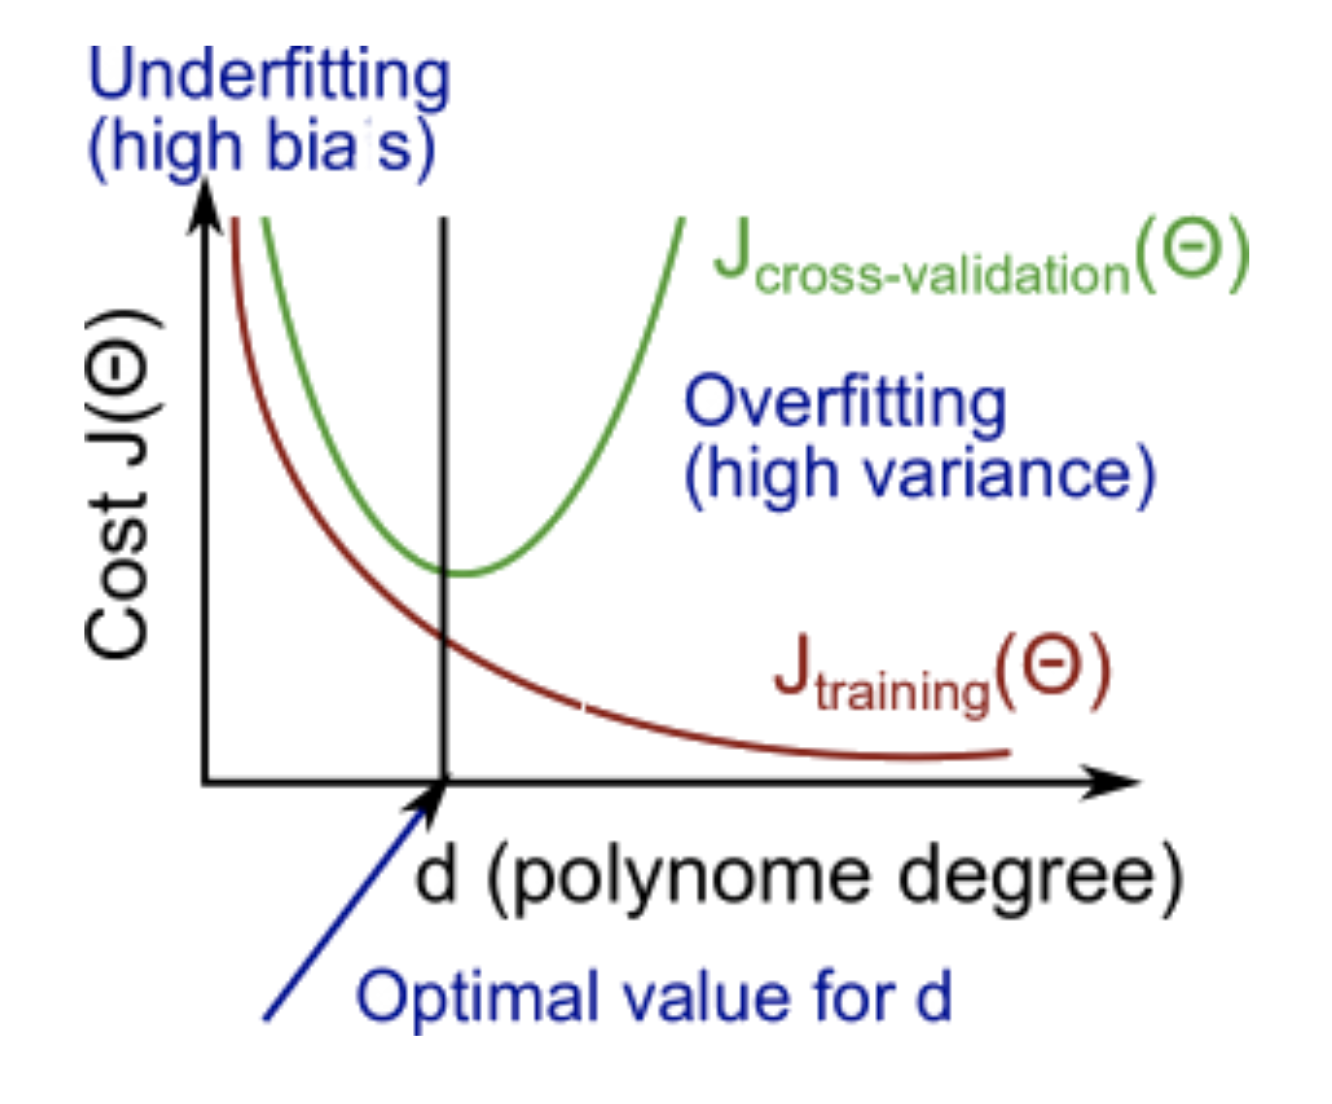
\includegraphics[width=0.5\textwidth]{fig/hv_hb}
	\caption{Optimal value for the degree \textit{d} of the polynomial}
\end{figure}

\section{Regularization and Bias/Variance}

We can see that as $ \lambda $ increases, our fit becomes more rigid. On the other hand, as $ \lambda $ approaches 0, we tend to overfit the data. So how do we choose our parameter $ \lambda $ to get it 'just right' ? In order to choose the model and the regularization term $ \lambda $, we need to:\\

\begin{enumerate}
\item Create a list of lambdas (i.e. $ \lambda \int $ \{0,0.01,0.02,0.04,0.08,0.16,0.32,0.64,1.28,2.56,5.12,10.24\});
\item Create a set of models with different degrees or any other variants.
\item Iterate through the $ \lambda $ and for each $ \lambda $ go through all the models to learn some $\Theta$.
\item Compute the cross validation error using the learned $\Theta$ (computed with $\lambda$) on the $J_{CV}(\Theta)$ without regularization or $ \lambda = 0$.
\item Select the best combo that produces the lowest error on the cross validation set.
\item Using the best combo $\Theta$ and $ \lambda $, apply it on $J_{test}(\Theta)$ to see if it has a good generalization of the problem.
\end{enumerate}


\section{Learning Curves}

Training an algorithm on a very few number of data points (such as 1, 2 or 3) will easily have 0 errors because we can always find a quadratic curve that touches exactly those number of points. Hence:

\begin{itemize}
\item As the training set gets larger, the error for a quadratic function increases.
\item The error value will plateau out after a certain m, or training set size.
\end{itemize}

\textbf{Experiencing high bias:}\\

\begin{tcolorbox}[width=\textwidth,colback={white},colbacktitle=white]
\textbf{Low training set size}: causes $ J_{train}(\Theta) $  to be low and $ J_{CV}(\Theta) $  to be high.\\

Large training set size: causes both $ J_{train}(\Theta) $  and $ J_{CV}(\Theta) $  to be high with $ J_{train}(\Theta) \approx  J_{CV}(\Theta) $ .
\end{tcolorbox}

If a learning algorithm is suffering from \textbf{high bias}, getting more training data will not (\textbf{by itself}) help much.\\

\begin{figure}[h!]
	\centering
	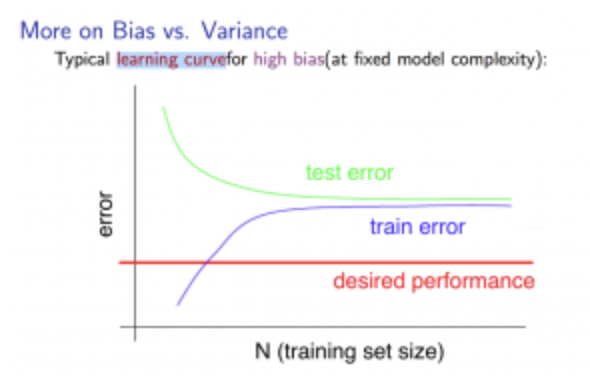
\includegraphics[width=0.6\textwidth]{fig/bias}
	\caption{High Bias}
\end{figure}

\pagebreak

\textbf{Experiencing high variance}:\\

\begin{tcolorbox}[width=\textwidth,colback={white},colbacktitle=white]
\textbf{Low training set size}: $ J_{train}(\Theta) $  will be low and $ J_{CV}(\Theta) $  to be high.\\

Large training set size: $ J_{train}(\Theta) $  increases with training set size and $ J_{CV}(\Theta) $  continues to decrease without leveling off. Also, $ J_{train}(\Theta) <  J_{CV}(\Theta) $ but the difference between them remains significant. .
\end{tcolorbox}

If a learning algorithm is suffering from \textbf{high variance}, getting more training data is \textbf{likely} to help.

\begin{figure}[h!]
	\centering
	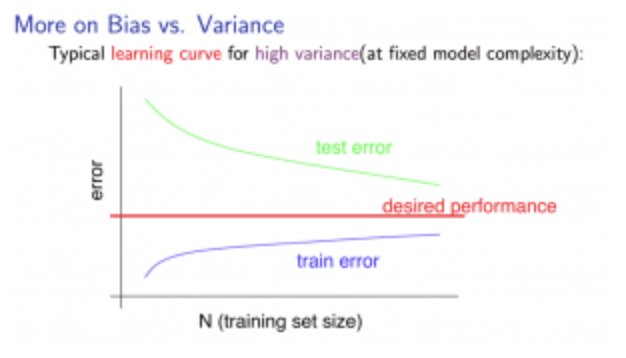
\includegraphics[width=0.6\textwidth]{fig/variance}
	\caption{High Variance}
\end{figure}

\pagebreak

\section{Deciding What to Do Next}

\begin{table}[h!]
	\caption{Decision process}
	\centering
	\begin{tabular}{|l|l|}
		\hline
		\multicolumn{1}{|c|}{\textbf{Fixes High BIAS}} & \multicolumn{1}{c|}{\textbf{Fixes High VARIANCE}} \\ \hline
		Adding features                                & Getting more training examples                    \\
		Adding polynomial features                     & Trying smaller sets of features                   \\
		Decreasing $\lambda$                           & Increasing $\lambda$                              \\ \hline
	\end{tabular}
\end{table}

\subsection{Diagnosing Neural Networks}

\begin{itemize}
\item A neural network with fewer parameters is prone to underfitting. It is also computationally cheaper.
\item A large neural network with more parameters is prone to overfitting. It is also computationally expensive. In this case you can use regularization (increase $\lambda$) to address the overfitting.
\end{itemize}

Using a single hidden layer is a good starting default. You can train your neural network on a number of hidden layers using your cross validation set. You can then select the one that performs best.

\subsection{Model Complexity Effects}

\begin{itemize}
\item Lower-order polynomials (low model complexity) have high bias and low variance. In this case, the model fits poorly consistently.
\item Higher-order polynomials (high model complexity) fit the training data extremely well and the test data extremely poorly. These have low bias on the training data, but very high variance.
\item In reality, we would want to choose a model somewhere in between, that can generalize well but also fits the data reasonably well.
\end{itemize}

\section{Prioritizing What to Work On}

\subsection{System Design Example}

Given a data set of emails, we could construct a vector for each email. Each entry in this vector represents a word. The vector normally contains 10,000 to 50,000 entries gathered by finding the most frequently used words in our data set. If a word is to be found in the email, we would assign its respective entry a 1, else if it is not found, that entry would be a 0. Once we have all our x vectors ready, we train our algorithm and finally, we could use it to classify if an email is a spam or not.

\begin{figure}[h!]
	\centering
	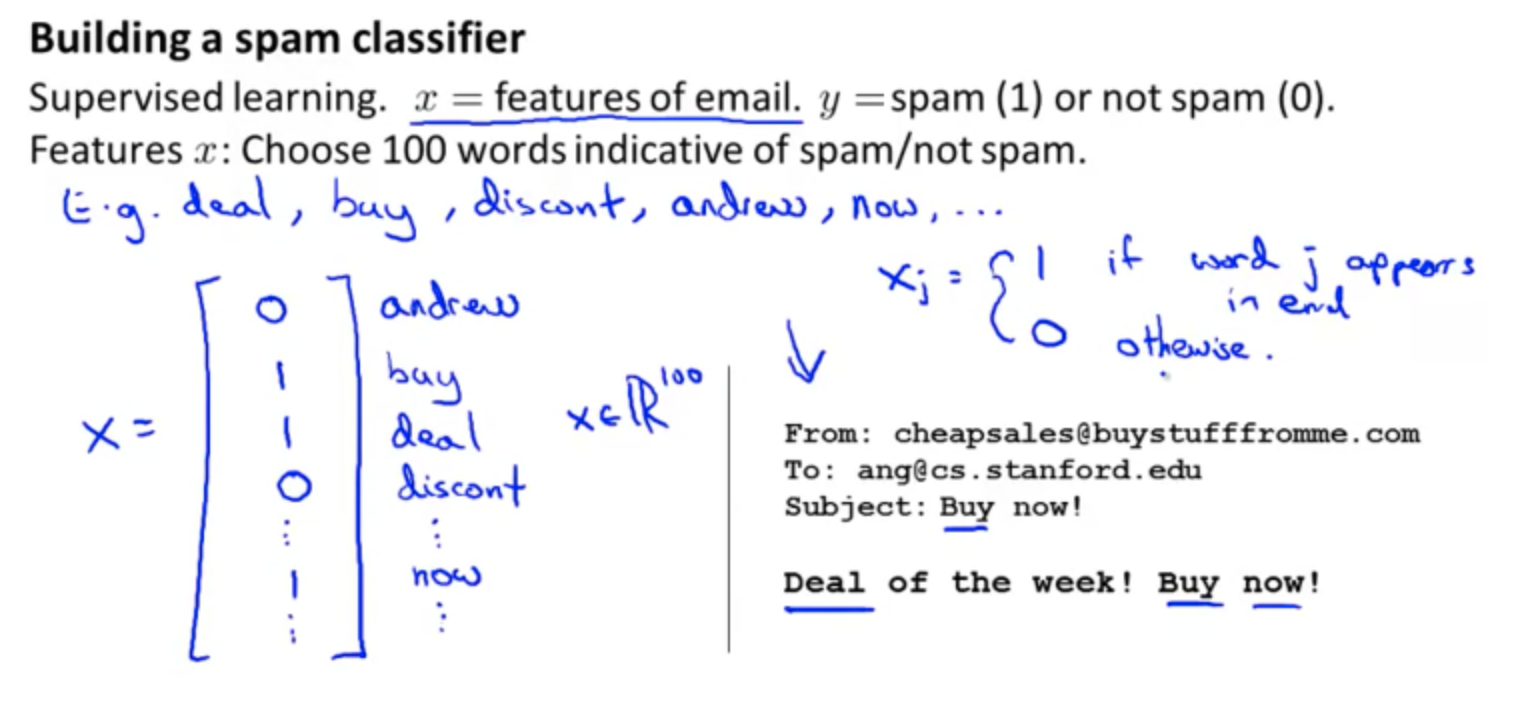
\includegraphics[width=1\textwidth]{fig/spam}
	\caption{Spam vector explanation}
\end{figure}

So how could you spend your time to improve the accuracy of this classifier?\\

\begin{itemize}
\item Collect lots of data (for example "honeypot" project but doesn't always work)
\item Develop sophisticated features (for example: using email header data in spam emails)
\item Develop algorithms to process your input in different ways (recognizing misspellings in spam).
\end{itemize}

It is difficult to tell which of the options will be most helpful.

\section{Error Analysis}

The recommended approach to solving machine learning problems is to:

\begin{enumerate}
\item Start with a simple algorithm, implement it quickly, and test it early on your cross validation data.
\item Plot learning curves to decide if more data, more features, etc. are likely to help.
\item Manually examine the errors on examples in the cross validation set and try to spot a trend where most of the errors were made.
\end{enumerate}

%For example, assume that we have 500 emails and our algorithm misclassifies a 100 of them. We could manually analyze the 100 emails and categorize them based on what type of emails they are. We could then try to come up with new cues and features that would help us classify these 100 emails correctly. Hence, if most of our misclassified emails are those which try to steal passwords, then we could find some features that are particular to those emails and add them to our model. We could also see how classifying each word according to its root changes our error rate.\\
%
%It is very important to get error results as a single, numerical value. Otherwise it is difficult to assess your algorithm's performance. For example if we use stemming, which is the process of treating the same word with different forms (fail/failing/failed) as one word (fail), and get a 3\% error rate instead of 5\%, then we should definitely add it to our model. However, if we try to distinguish between upper case and lower case letters and end up getting a 3.2\% error rate instead of 3\%, then we should avoid using this new feature. Hence, we should try new things, get a numerical value for our error rate, and based on our result decide whether we want to keep the new feature or not.
%
%\section{Skewed data}
%
%A data is called as skewed when curve appears distorted or skewed either to the left or to the right, in a statistical distribution. In a normal distribution, the graph appears symmetry meaning that there are about as many data values on the left side of the median as on the right side.\\
%
%In case of normal distribution, the mean, median and model are approximately closer. These three are all measures of the center of a data. The skewness of the data can be determined by how these quantities are related to one another.\\
%
%\subsection{Error metrics for skewed classes}
%
%Consider the problem of cancer classification, where we have features of medical patients and we want to decide whether or not they have cancer. So this is like the malignant versus benign tumor classification.\\
%
%Let's say \textbf{y equals 1} if the patient has cancer and \textbf{y equals 0} if they do not. We have trained the progression classifier and let's say we test our classifier on a test set and find that we get 1 percent error. So, we're making 99\% correct diagnosis. Seems like a really impressive result. We're correct 99\% percent of the time.\\
%
%But now, let's say we find out that only 0.5 percent of patients in our training test sets actually have cancer. So only half a percent of the patients that come through our screening process have cancer. In this case, the 1\% error no longer looks so impressive.\\
%
%So this setting of when the ratio of positive to negative examples is very close to one of two extremes, where, in this case, the number of positive examples is much, much smaller than the number of negative examples because y equals one so rarely, this is what we call the case of skewed classes.\\
%
%We just have a lot more of examples from one class than from the other class. And by just predicting y equals 0 all the time, or maybe our predicting y equals 1 all the time, an algorithm can do pretty well. So the problem with using classification error or classification accuracy as our evaluation metric is the following.\\
%
%Let's say you have one joining algorithm that's getting 99.2\% accuracy. So, that's a 0.8\% error. Let's say you make a change to your algorithm and you now are getting 99.5\% accuracy. That is 0.5\% error.\\
%
%If you have very skewed classes it becomes much harder to use just classification accuracy, because you can get very high classification accuracies or very low errors, and it's not always clear if doing so is really improving the quality of your classifier because predicting y equals 0 all the time doesn't seem like a particularly good classifier.\\
%Start transcript at 3 minutes 53 seconds3:53
%But just predicting y equals 0 more often can bring your error down to, you know, maybe as low as 0.5%. When we're faced with such a skewed classes therefore we would want to come up with a different error metric or a different evaluation metric. One such evaluation metric are what's called precision recall.
%Start transcript at 4 minutes 15 seconds4:15
%Let me explain what that is.
%Start transcript at 4 minutes 17 seconds4:17
%Let's say we are evaluating a classifier on the test set. For the examples in the test set the actual
%Start transcript at 4 minutes 25 seconds4:25
%class of that example in the test set is going to be either one or zero, right, if there is a binary classification problem.
%Start transcript at 4 minutes 33 seconds4:33
%And what our learning algorithm will do is it will, you know, predict some value for the class and our learning algorithm will predict the value for each example in my test set and the predicted value will also be either one or zero.
%Start transcript at 4 minutes 50 seconds4:50
%So let me draw a two by two table as follows, depending on a full of these entries depending on what was the actual class and what was the predicted class. If we have an example where the actual class is one and the predicted class is one then that's called
%Start transcript at 5 minutes 7 seconds5:07
%an example that's a true positive, meaning our algorithm predicted that it's positive and in reality the example is positive. If our learning algorithm predicted that something is negative, class zero, and the actual class is also class zero then that's what's called a true negative. We predicted zero and it actually is zero.
%Start transcript at 5 minutes 27 seconds5:27
%To find the other two boxes, if our learning algorithm predicts that the class is one but the
%Start transcript at 5 minutes 34 seconds5:34
%actual class is zero, then that's called a false positive.
%Start transcript at 5 minutes 39 seconds5:39
%So that means our algorithm for the patient is cancelled out in reality if the patient does not.
%Start transcript at 5 minutes 44 seconds5:44
%And finally, the last box is a zero, one. That's called a false negative because our algorithm predicted zero, but the actual class was one.
%Start transcript at 5 minutes 57 seconds5:57
%And so, we have this little sort of two by two table based on what was the actual class and what was the predicted class.
%Start transcript at 6 minutes 7 seconds6:07
%So here's a different way of evaluating the performance of our algorithm. We're going to compute two numbers. The first is called precision - and what that says is,
%Start transcript at 6 minutes 17 seconds6:17
%of all the patients where we've predicted that they have cancer,
%Start transcript at 6 minutes 20 seconds6:20
%what fraction of them actually have cancer?
%Start transcript at 6 minutes 24 seconds6:24
%So let me write this down, the precision of a classifier is the number of true positives divided by
%Start transcript at 6 minutes 32 seconds6:32
%the number that we predicted
%Start transcript at 6 minutes 37 seconds6:37
%as positive, right?
%Start transcript at 6 minutes 39 seconds6:39
%So of all the patients that we went to those patients and we told them, "We think you have cancer." Of all those patients, what fraction of them actually have cancer? So that's called precision. And another way to write this would be true positives and then in the denominator is the number of predicted positives, and so that would be the sum of the, you know, entries in this first row of the table. So it would be true positives divided by true positives. I'm going to abbreviate positive as POS and then plus false positives, again abbreviating positive using POS.
%Start transcript at 7 minutes 20 seconds7:20
%So that's called precision, and as you can tell high precision would be good. That means that all the patients that we went to and we said, "You know, we're very sorry. We think you have cancer," high precision means that of that group of patients most of them we had actually made accurate predictions on them and they do have cancer.
%Start transcript at 7 minutes 38 seconds7:38
%The second number we're going to compute is called recall, and what recall say is, if all the patients in, let's say, in the test set or the cross-validation set, but if all the patients in the data set that actually have cancer,
%Start transcript at 7 minutes 52 seconds7:52
%what fraction of them that we correctly detect as having cancer. So if all the patients have cancer, how many of them did we actually go to them and you know, correctly told them that we think they need treatment.
%Start transcript at 8 minutes 5 seconds8:05
%So, writing this down, recall is defined as the number of positives, the number of true positives, meaning the number of people that have cancer and that we correctly predicted have cancer
%Start transcript at 8 minutes 20 seconds8:20
%and we take that and divide that by, divide that by the number of actual positives,
%Start transcript at 8 minutes 31 seconds8:31
%so this is the right number of actual positives of all the people that do have cancer. What fraction do we directly flag and you know, send the treatment.
%Start transcript at 8 minutes 40 seconds8:40
%So, to rewrite this in a different form, the denominator would be the number of actual positives as you know, is the sum of the entries in this first column over here.
%Start transcript at 8 minutes 50 seconds8:50
%And so writing things out differently, this is therefore, the number of true positives, divided by
%Start transcript at 8 minutes 59 seconds8:59
%the number of true positives
%Start transcript at 9 minutes 2 seconds9:02
%plus the number of
%Start transcript at 9 minutes 6 seconds9:06
%false negatives.
%Start transcript at 9 minutes 9 seconds9:09
%And so once again, having a high recall would be a good thing.
%Start transcript at 9 minutes 14 seconds9:14
%So by computing precision and recall this will usually give us a better sense of how well our classifier is doing.
%Start transcript at 9 minutes 21 seconds9:21
%And in particular if we have a learning algorithm that predicts y equals zero all the time, if it predicts no one has cancer, then this classifier will have a recall equal to zero, because there won't be any true positives and so that's a quick way for us to recognize that, you know, a classifier that predicts y equals 0 all the time, just isn't a very good classifier. And more generally, even for settings where we have very skewed classes, it's not possible for an algorithm to sort of "cheat" and somehow get a very high precision and a very high recall by doing some simple thing like predicting y equals 0 all the time or predicting y equals 1 all the time. And so we're much more sure that a classifier of a high precision or high recall actually is a good classifier, and this gives us a more useful evaluation metric that is a more direct way to actually understand whether, you know, our algorithm may be doing well.
%Start transcript at 10 minutes 21 seconds10:21
%So one final note in the definition of precision and recall, that we would define precision and recall, usually we use the convention that y is equal to 1, in the presence of the more rare class. So if we are trying to detect. rare conditions such as cancer, hopefully that's a rare condition, precision and recall are defined setting y equals 1, rather than y equals 0, to be sort of that the presence of that rare class that we're trying to detect. And by using precision and recall, we find, what happens is that even if we have very skewed classes, it's not possible for an algorithm to you know, "cheat" and predict y equals 1 all the time, or predict y equals 0 all the time, and get high precision and recall. And in particular, if a classifier is getting high precision and high recall, then we are actually confident that the algorithm has to be doing well, even if we have very skewed classes.
%Start transcript at 11 minutes 18 seconds11:18
%So for the problem of skewed classes precision recall gives us more direct insight into how the learning algorithm is doing and this is often a much better way to evaluate our learning algorithms, than looking at classification error or classification accuracy, when the classes are very skewed.

\chapter{Support Vector Machine (SVM)}

Support vector machine is another simple algorithm that every machine learning expert should have in his/her arsenal. Support vector machine is highly preferred by many as it produces significant accuracy with less computation power. Support Vector Machine, abbreviated as SVM can be used for both regression and classification tasks. But, it is widely used in classification objectives.\\

If we look at the cost function of logistic regression, what we'll find is that each example (x,y) contributes a term to the overall cost function.\\

\begin{center}
	$$J(\theta) = -\frac{1}{m}\sum_{i=1}^{m}\left[y^{(i)}\cdot log(h_\theta(x^{(i)})) +(1-y^{(i)})\cdot log(1-h_\theta(x^{(i)}))\right] $$
\end{center}

When y is equal to one we get the left term: 

\begin{center}
\Large{
$- y \cdot log \frac{1}{1 + e^{ - \theta^T x}} $}
\end{center}

And if we plot this function as a function of z, what we find is that we get this curve shown on the lower left of the next figure. And thus, we also see that when z is equal to large, that is, when theta transpose x is large, that corresponds to a value of z that gives us a fairly small value, a very small contribution to the consumption. And this kinda explains why, when logistic regression sees a positive example, with y=1, it tries to set theta transport x to be very large because that corresponds to this term, in the cross function, being small. \\

\begin{figure}[h!]
	\centering
	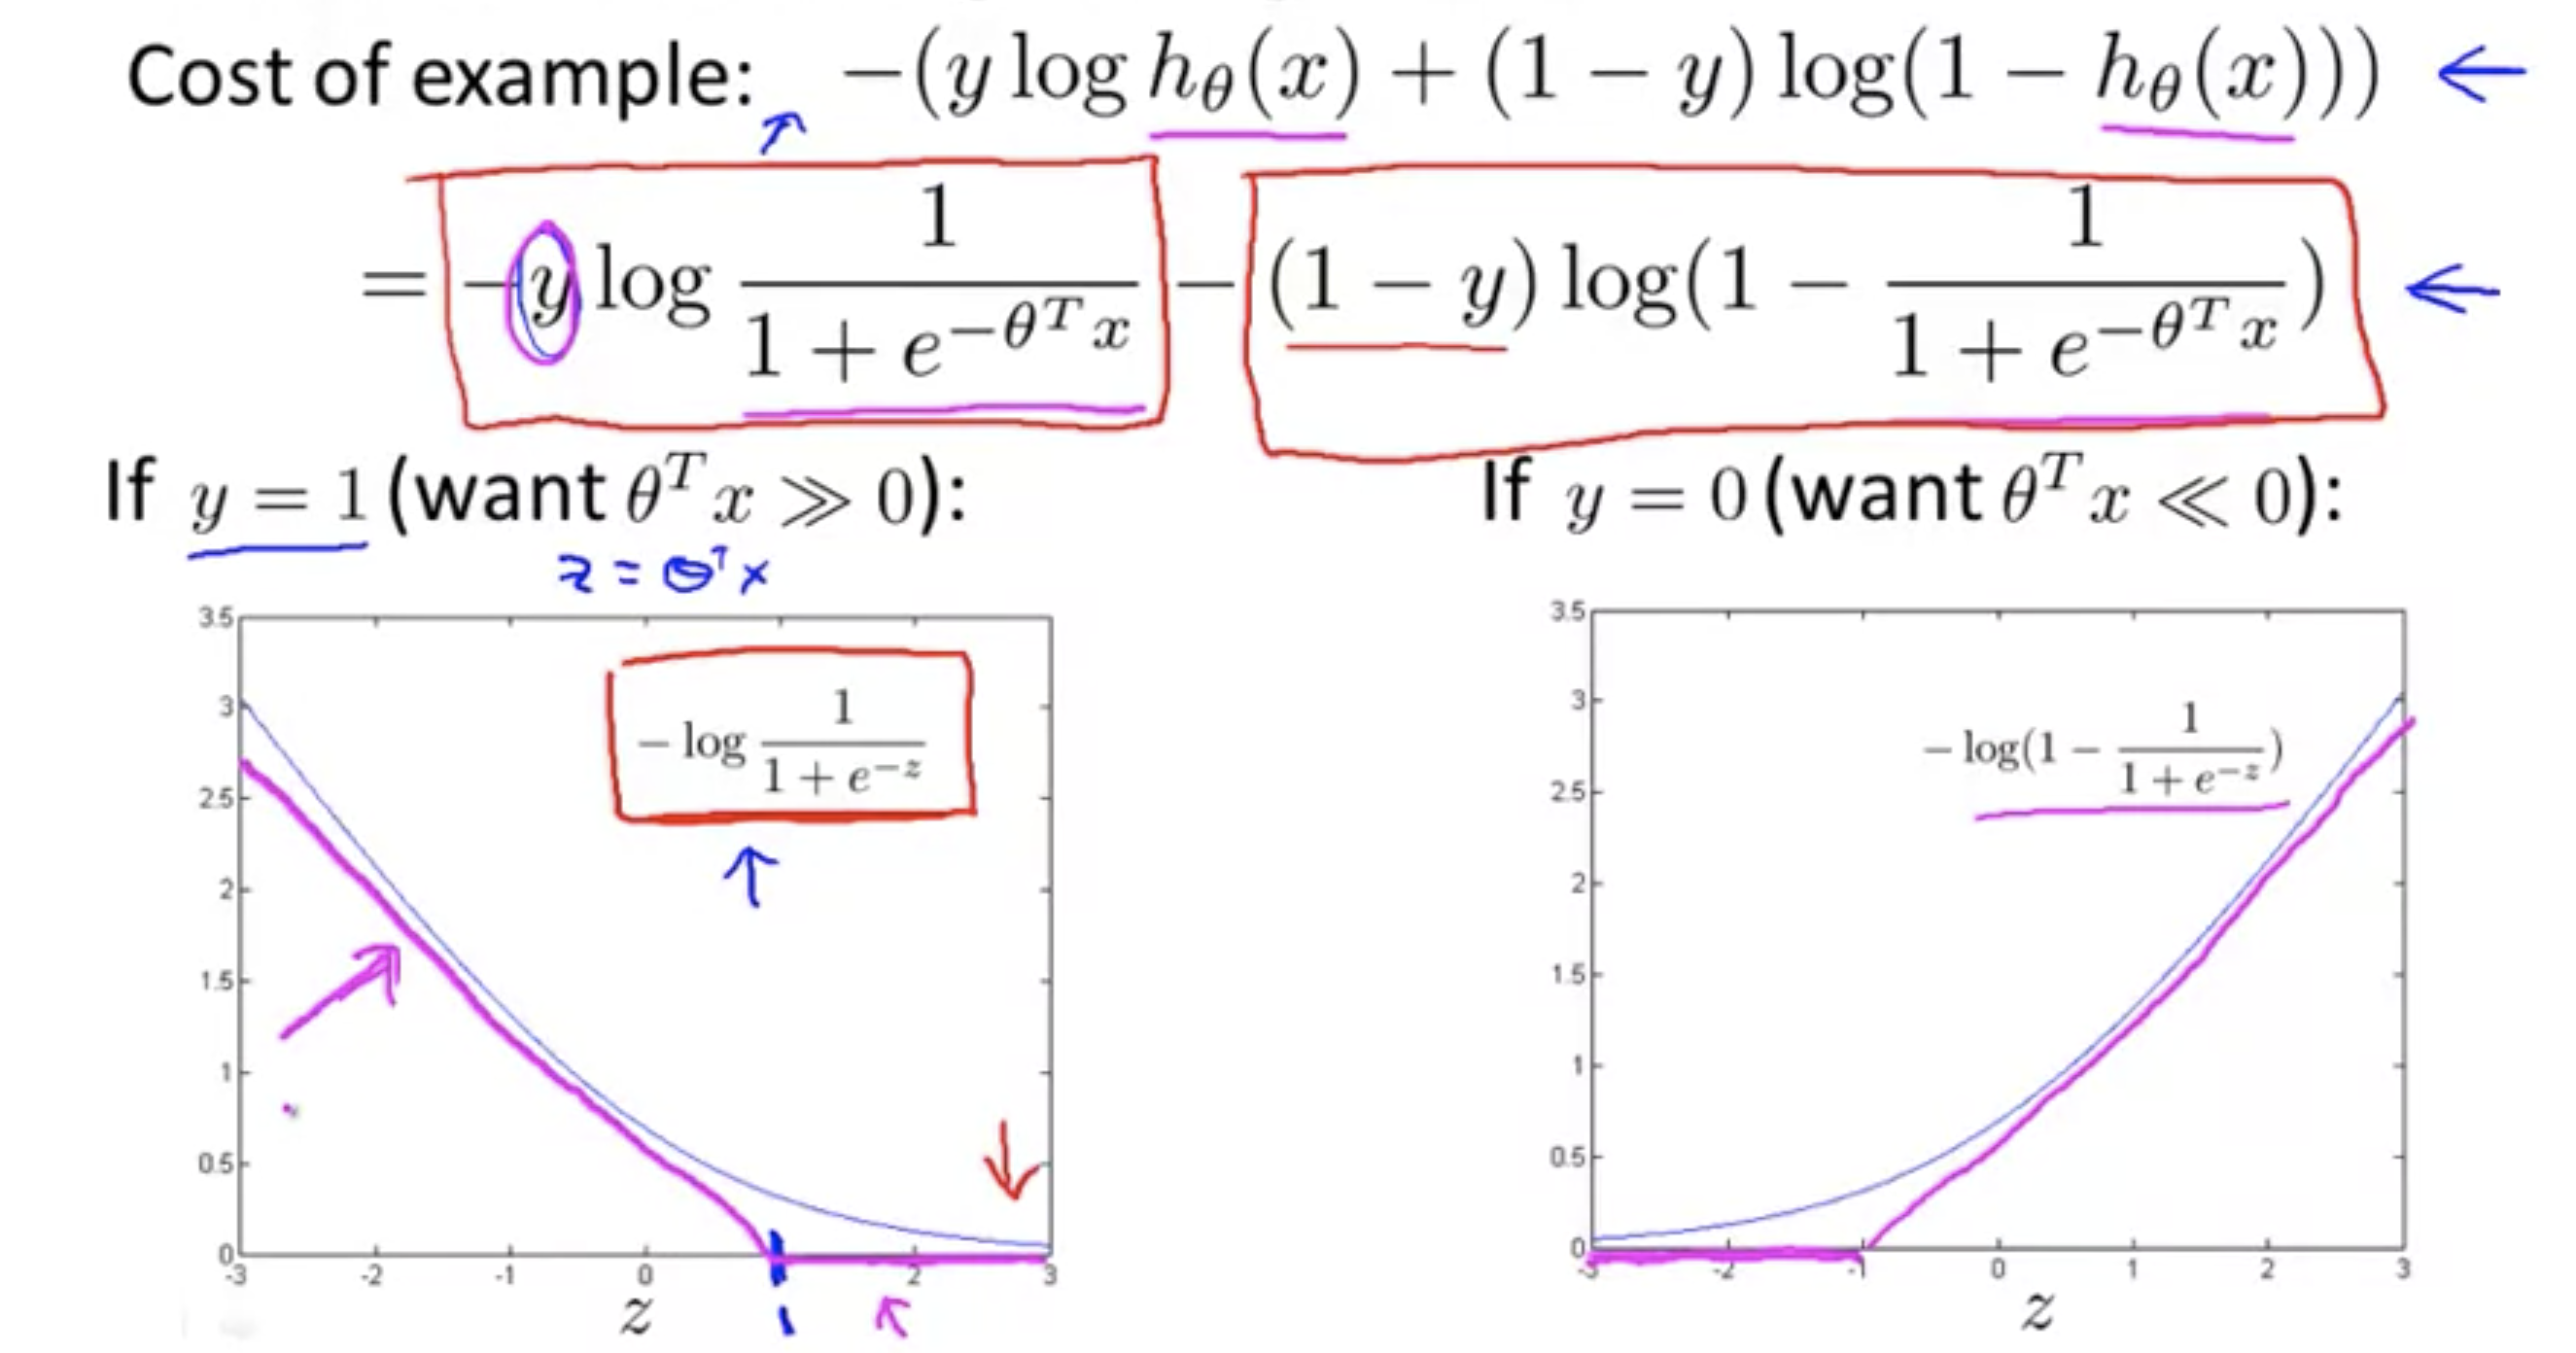
\includegraphics[width=0.7\textwidth]{fig/SVM}
	\caption{Logistic Cost example}
	\label{fig:svm}
\end{figure}

\pagebreak

Now, to fill the support vector machine, here's what we're going to do. We're gonna take this cross function, this on the left, and modify it a little bit. The new pass functions (drew in magenta) can be flat from here on out, and then we draw something that grows as a straight line, similar to logistic regression. But this is going to be a straight line at this portion. So the curve that I just drew in magenta, and the curve I just drew in purple and magenta, so it's pretty close approximation to the cross function used by logistic regression. Except it is now made up of two line segments, there's this flat portion on the right, and then there is this straight line portion on the left. \\

That's the new cost function we're going to use for when y is equal to one, and you can imagine it should do something pretty similar to logistic regression. But turns out, that this will give the support vector machine computational advantages and give us, later on, an easier optimization problem.\\

The other case is if y is equal to zero. In that case, if you look at the cost, then only the second term will apply because the first term goes away, right? If y is equal to zero, then you have a zero here, so you're left only with the second term of the expression. And for the support vector machine, once again, we're going to replace this blue line with something similar and at the same time we replace it with a new cost, this flat out here, this 0 out here. And that then grows as a straight line.\\

We're going to call this function on the left $ Cost_1(z) $ and this function of the right we're gonna call $ Cost_0(z) $. \\

The subscript just refers to the cost corresponding to when y is equal to 1, versus when y Is equal to zero.\\

So we have this SVM Cost function :

\begin{equation}
min_\theta  \hspace{0.2cm} C \sum_{i=1}^{m}\left( y^{(i)} Cost_1(\theta^T x) +(1- y^{(i)}) Cost_0(\theta^T x) \right) + \frac{1}{2}  \sum_{i=1}^{n} \theta_j^2
\end{equation}

\section{Large Margin Intuition}

Let's think about what it takes to make these cost functions small. If you have a positive example, (y is equal to 1), then $ Cost_1(z) $ is zero only when $ z \geq 1 $. So in other words, if you have a positive example, we really want theta transpose x to be greater than or equal to 1 and conversely if y is equal to zero, look this $ Cost_0(z) $ then it's only in this region where $ z \leq -1 $ we have the cost is zero as z is equals to zero.

\begin{figure}[h!]
	\centering
	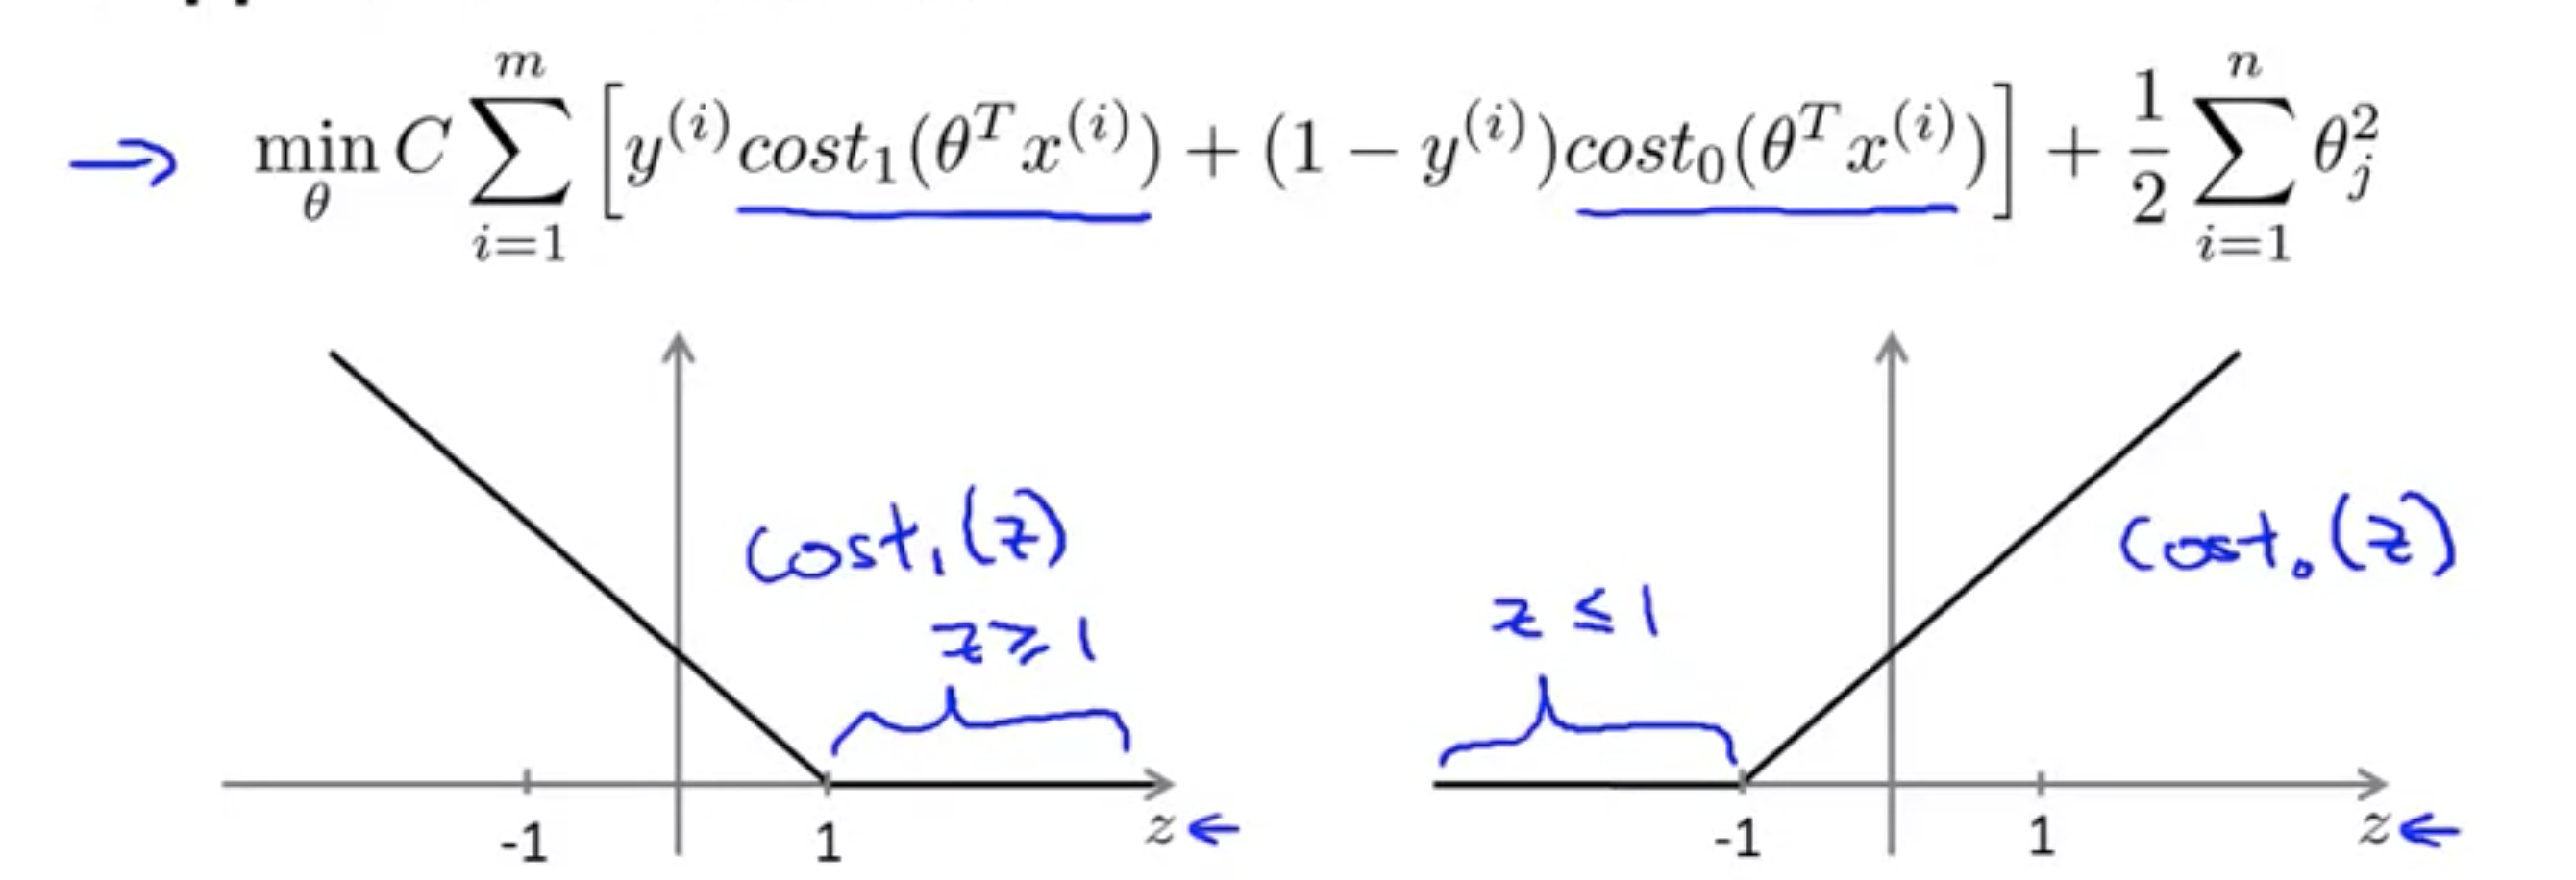
\includegraphics[width=0.7\textwidth]{fig/LMI_SVM_0}
	\caption{Large Marge Intuition}
	\label{fig:lmisvm0}
\end{figure}

In logistic regression, we take the output of the linear function and squash the value within the range of [0,1] using the sigmoid function. If the squashed value is greater than a threshold value(0.5) we assign it a label 1, else we assign it a label 0. In SVM, we take the output of the linear function and if that output is greater than 1, we identify it with one class and if the output is -1, we identify is with another class. Since the threshold values are changed to 1 and -1 in SVM, we obtain this reinforcement range of values([-1,1]) which acts as margin.\\

Using these support vectors, we maximize the margin of the classifier. Deleting the support vectors will change the position of the hyperplane (hypotheses). These are the points that help us build our SVM.

\begin{figure}[h!]
	\centering
	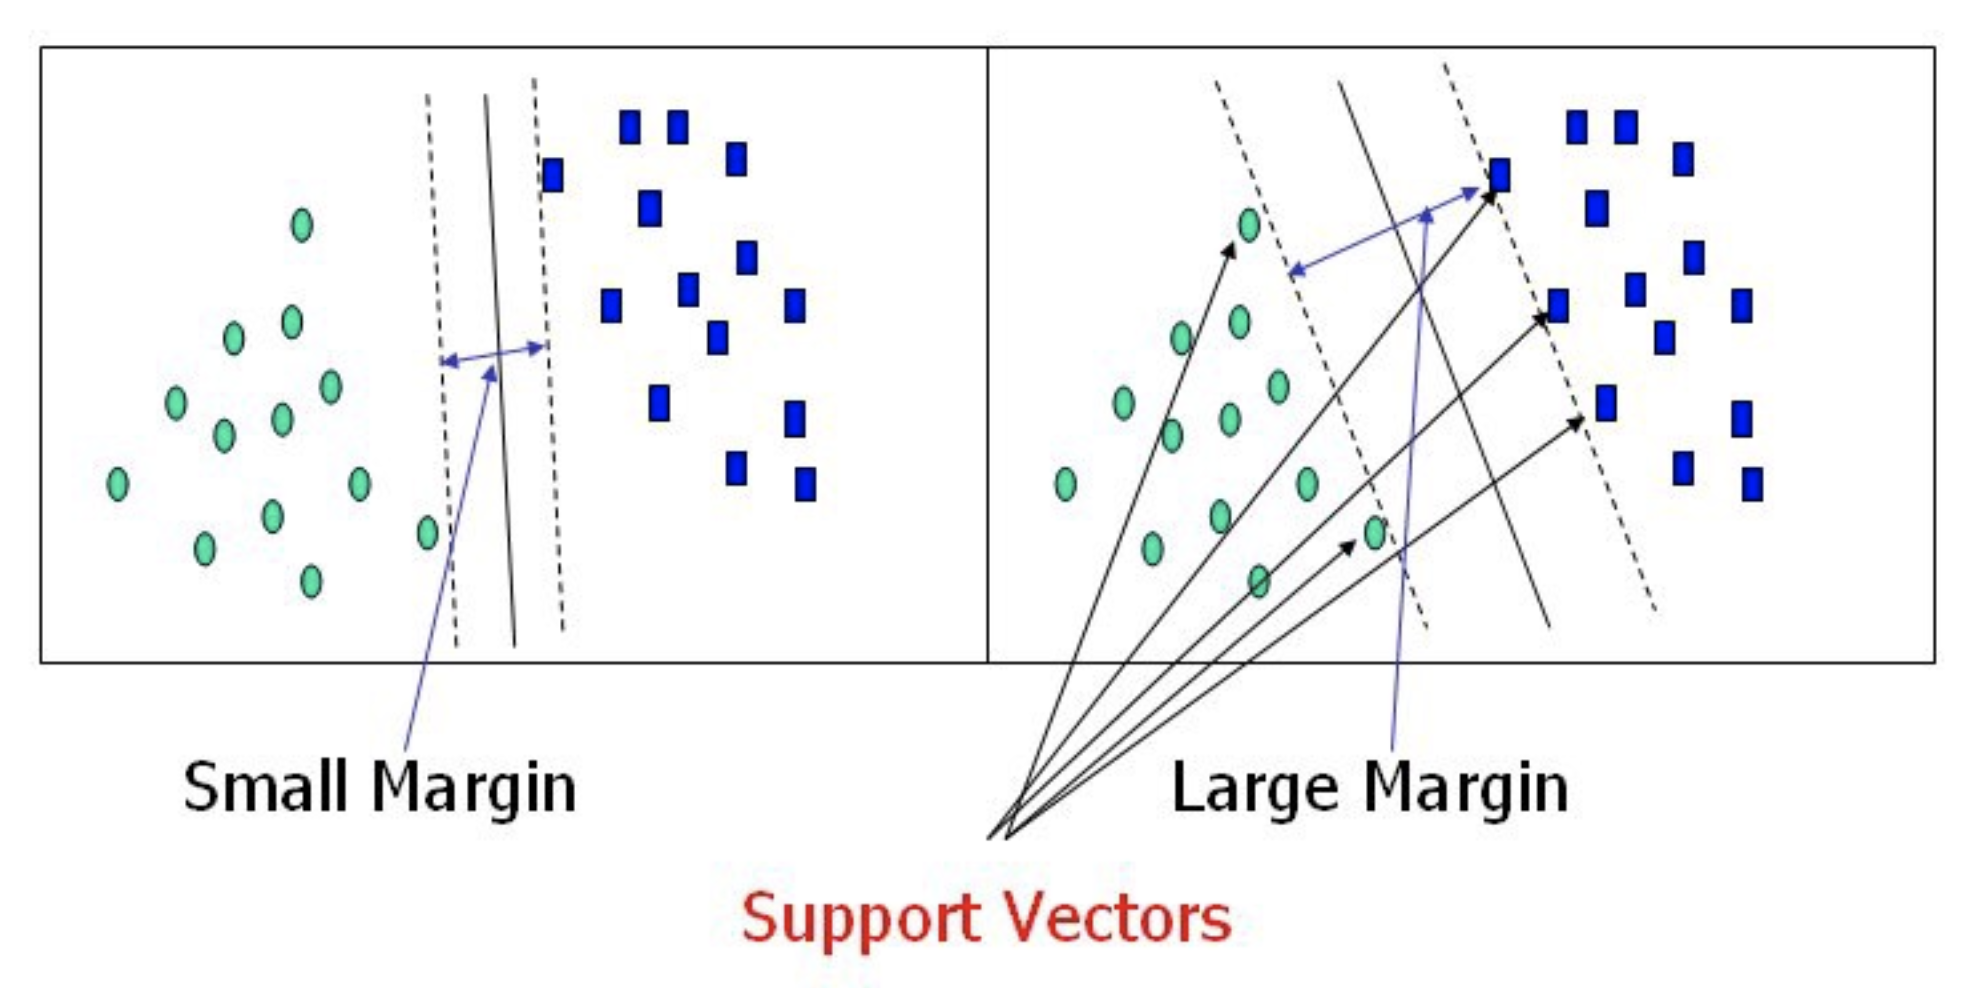
\includegraphics[width=0.7\textwidth]{fig/LMI_SVM}
	\caption{Large Marge Intuition}
	\label{fig:lmisvm}
\end{figure}

\end{document}